\documentclass{cmspaper}
\usepackage{placeins}
\usepackage{subfig}
\usepackage{graphicx}
\usepackage{lineno}

\usepackage[dvipsnames]{xcolor}
\usepackage[utf8]{inputenc}
\usepackage[english]{babel}
%\usepackage{csquotes}

\usepackage [english]{babel}
\usepackage [autostyle, english = american]{csquotes}
\MakeOuterQuote{"}
%\usepackage[backend=biber,style=ieee,citestyle=numeric-comp,sorting=none]{biblatex}
%usepackage[backend=biber,style=chem-angew,citestyle=numeric-comp,sorting=none]{biblatex}
%\ package 'overpic' for plot test manipulation
%\usepackage[backend=biber,style=alphabetic,sorting=ynt]{biblatex}
\usepackage[backend=biber,style=numeric,sorting=none]{biblatex}
\addbibresource{jwkbiblio.bib}

\begin{document}

%==============================================================================
% title page for few authors

\begin{titlepage}

% select one of the following and type in the proper number:
%\cmsnote{2022/075}
%\internalnote{2005/000}
%\conferencereport{2005/000}
\title{Paper Draft}
\date{30 May 2025}

\title{Studies of ECAL Timing Reconstruction }

\begin{Authlist}
    %A.~Author, B.~Author, C.~Author\Aref{a}
       %\Instfoot{cern}{CERN, Geneva, Switzerland}
    J.~King, N.~Minafra, C.~Rogan
       \Instfoot{ku}{University of Kansas, Lawrence KS, USA}
       %\Instfoot{ieph}{Institute of Experimental Physics, Hepcity, Wonderland}
\end{Authlist}

% if needed, use the following:
\collaboration{CMS collaboration}

\begin{abstract}
\centering
One of the most exciting elements of the future CMS detector anticipated for the High Luminosity LHC (HL-LHC) era, will be the incorporation of precision timing. A combination of new sub-detectors (MTD, HGCAL) and dedicated upgrades to existing detectors, such as the ECAL, will facilitate 4D reconstruction of events. 4D reconstruction methods will provide new tools for both pile-up suppression and a range of new experimental techniques to probing physics signatures and long-lived particles. To facilitate the incorporation of precision timing in the HL-LHC era, studies of the ECAL timing reconstruction were conducted and a new time reconstruction, the Cross Correlation Time Algorithm ( CC ), was developed. The CC algorithm mitigates the effects of out-of-time pileup on the ECAL time reconstruction by leveraging the existing, pile-up aware, ECAL energy reconstruction method. In order to measure the performance of this new algorithm, refinements to existing methods to determine timing resolution and new methods to determine approximate GEN truth times were developed. The CC algorithm is shown to improve the single crystal resolution by $\sim$30 ps over the Run II default method and is expected to achieve analysis relevant E/Gamma object resolutions of $\sim$100 ps, compared to $\sim$300 ps typical in Run II. With the utilization of the CC algorithm we expect comparable, if not improved, resolutions in Run III.

%The time resolutions achievable with the CC algorithm will improve the sensitivity of LLP searches, allowing them to be sensitive to ctaus  down to ~ 3 cm from the ~ 10 cm achievable currently.  

%While not yet approaching the planned future precision and coverage for timing, recent improvements to the ECAL timing reconstruction using a new algorithm, the cross-correlation method ( CC ), will allow for some parts of this 4D future to be realized in Run III. 

%With the improvements provided by the CC algorithm in  mind, a method to time stamp vertices by constructing a jet time is being studied.  This method shows the potential to match the time resolution achievable to real world physics objects in the ECAL that, with the CC algorithm, would allow the time stamping of vertices with ~ 100 ps resolution using the current detector in Run II. With this method we expect to time stamp vertices to  a comparable, if not improved, resolution in Run III.
\end{abstract} 

% if needed, use the following:
%\conference{Presented at {\it Physics Rumours}, Coconut Island, April 1, 2005}
%\submitted{Submitted to {\it Physics Rumours}}
\note{Preliminary version}
  
\end{titlepage}

\setcounter{page}{2}%JPP
\tableofcontents
\pagebreak
\linenumbers

\section{Introduction \label{sec:intro}}
The Compact Muon Solenoid (CMS) experiment at the Large Hadron Collider (LHC) is designed to explore particle physics at the TeV energy scale.
The electromagnetic calorimeter (ECAL) plays a central role in this program by providing precise energy measurements for electrons and photons produced in proton--proton collisions~\cite{Chatrchyan:1129810}.
In addition to its primary energy measurement capability, the ECAL can achieve excellent timing resolution, enabled by the fast scintillation response of lead tungstate (PbWO$_4$) crystals, the characteristics of the front-end electronics, and the high-frequency sampling of the readout system.

Future operation of the LHC, including Run~III and the High-Luminosity LHC (HL-LHC) era~\cite{Apollinari:2015wtw}, will significantly increase the instantaneous luminosity relative to previous runs.
While these conditions will allow the accumulation of unprecedented integrated luminosity, they will also substantially increase the number of overlapping proton--proton interactions per bunch crossing, commonly referred to as pileup (PU).
To mitigate the impact of pileup on event reconstruction, both the CMS and ATLAS experiments are pursuing the integration of precision timing information into their detectors~\cite{Butler:2019rpu,Morgenstern:2019xto}.
Within CMS, this strategy includes new dedicated timing detectors as well as upgrades to existing subsystems, such as the ECAL, with the goal of achieving time resolutions at the level of approximately 30\,ps in the HL-LHC era~\cite{Bruneliere:2006ra}.

The CMS ECAL is a hermetic homogeneous calorimeter composed of 75\,848 PbWO$_4$ scintillating crystals arranged in a barrel section and two endcap sections~\cite{cmstdr}.
The crystals are characterized by a high density, short radiation length, and small Moli\`ere radius, enabling a compact and highly granular detector geometry.
Scintillation light produced by electromagnetic showers is detected using avalanche photodiodes in the barrel and vacuum phototriodes in the endcaps~\cite{Bayatian:2006nff}.
The scintillation time profile of PbWO$_4$ is well matched to the LHC bunch crossing interval, with the majority of the emitted light collected within 25\,ns.

While the primary function of the ECAL is the measurement of electromagnetic energy, the achievable timing resolution has a direct impact on both energy reconstruction and physics sensitivity.
ECAL timing information is used to suppress backgrounds with broad or noncollision-related time distributions, including contributions from cosmic rays, beam halo muons, electronic noise, secondary interactions in detector material, and out-of-time proton--proton collisions~\cite{Bruneliere:2006ra}.
In addition, precise timing measurements significantly enhance sensitivity to searches for long-lived particles, where delayed decays can produce measurable shifts in the arrival time of photons and electrons at the calorimeter.

The reconstruction of ECAL time is sensitive to scintillation signals originating from pileup interactions, particularly those occurring in bunch crossings preceding or following the hard-scatter interaction of interest.
Such contributions, referred to as out-of-time pileup (OOT-PU), distort the reconstructed pulse shape and degrade the time resolution.
As luminosity increases, OOT-PU becomes a dominant limitation of existing timing reconstruction techniques.
Since ECAL timing is also used to reject backgrounds arising from OOT-PU, degradation in timing performance can adversely affect a wide range of physics measurements.

To address these challenges, it is essential to develop timing reconstruction methods that are robust against OOT-PU.
In this paper, a cross-correlation (CC) timing algorithm is introduced that exploits the pileup-aware ECAL energy reconstruction to mitigate the impact of out-of-time signals on the time measurement.
The performance of this algorithm is evaluated using data and simulation, and compared to the default Run~II ratio-based time reconstruction.
Improvements in single-crystal and object-level timing resolution are demonstrated, with direct relevance for Run~III operation and as a foundation for future precision timing applications at CMS.

The paper is organized as follows.
Section~\ref{sec:algo} introduces the ECAL time reconstruction algorithms, including the ratio-based reconstruction used in Run~II and the cross-correlation (CC) method developed to mitigate out-of-time pileup.
The timing performance, resolution methodology, and calibration strategy are presented in Section~\ref{sec:res}, together with results obtained in data and simulation.
The main conclusions are summarized in Section~\ref{sec:conclusion}.
%redone
\FloatBarrier

\section{ECAL Time Reconstruction Algorithms \label{sec:algo}}
The ECAL measures both the energy deposited by incident particles and the time at which that energy is deposited.
In both cases, these quantities are inferred from the scintillation light pulse produced when an incident particle interacts with a PbWO$_4$ crystal.
An electromagnetic particle incident on a PbWO$_4$ crystal initiates an electromagnetic shower consisting primarily of electrons, positrons, and photons.
As the shower particles lose energy through ionization, scintillation centers in the crystal are excited and subsequently de-excite, emitting scintillation light at a characteristic wavelength.
The total emitted light is proportional to the energy deposited by the incident particle.

The scintillation signal is amplified and shaped by the front-end readout electronics, which define a characteristic pulse shape~\cite{Karimaki:368412}.
For a given crystal channel, this pulse shape is stable and well characterized.
Ten consecutive samples of the pulse amplitude are recorded for each event.
Figure~\ref{tec_pulseshape} shows a typical ECAL pulse shape after amplification (solid line), together with the ten discrete amplitude samples (points).
The normalized pulse amplitude, $A/A_{\mathrm{max}}$, is shown as a function of the time difference $T - T_{\mathrm{max}}$, where $T_{\mathrm{max}}$ denotes the time at which the pulse reaches its maximum value.

\begin{figure}[htbp]
\begin{center}
\resizebox{0.75\linewidth}{!}{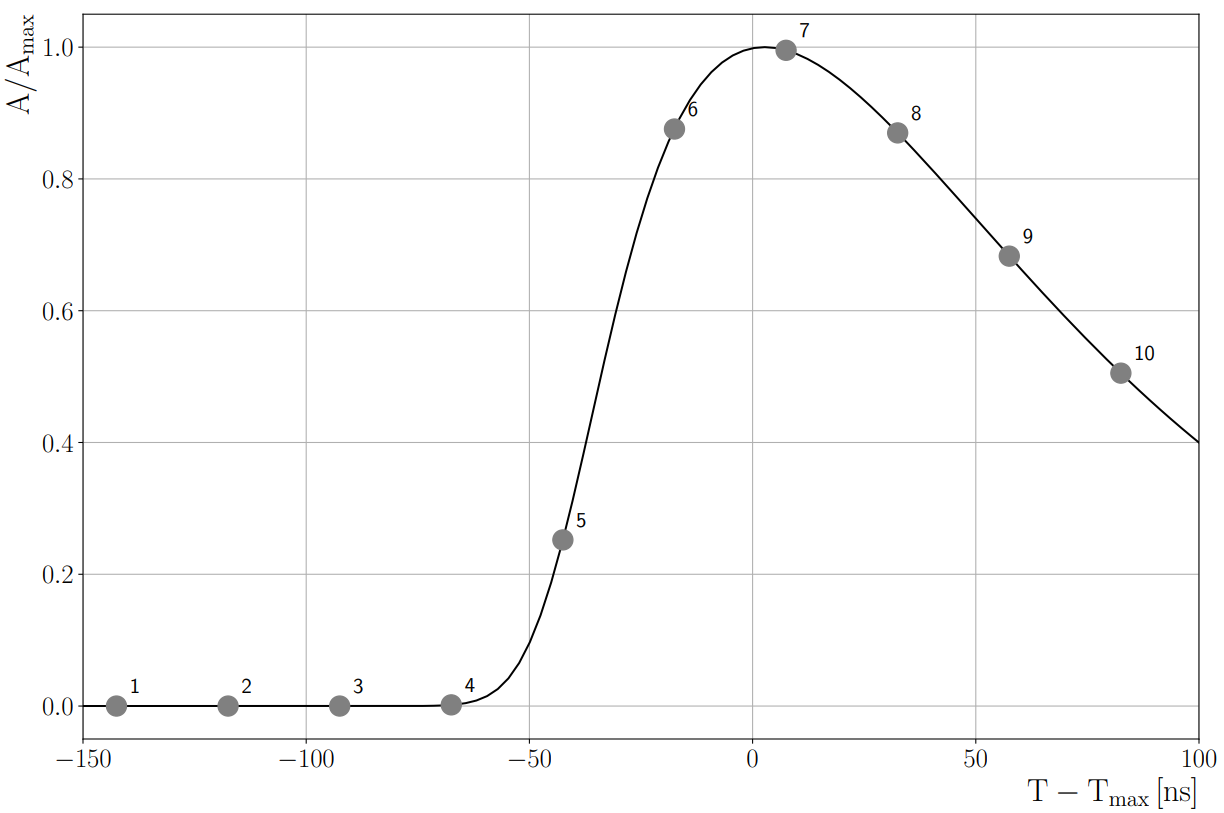
\includegraphics{fig/sec_reco/pulse_template.png}}
\caption{Typical ECAL pulse shape as a function of the difference between the ADC sample time $T$ and the pulse maximum time $T_{\mathrm{max}}$.
The amplitude $A$ is normalized to the maximum pulse amplitude $A_{\mathrm{max}}$.
The solid line shows the expected pulse shape after amplification, while the points indicate the ten discrete samples recorded for a single event, with the pedestal subtracted.}
\label{tec_pulseshape}
\end{center}
\end{figure}

During LHC Run~II (2015--2018), the instantaneous luminosity increased significantly relative to Run~I, resulting in a substantial rise in the number of interactions per bunch crossing (BX).
At the LHC, proton beams are composed of discrete bunches confined in radio-frequency buckets, and a \emph{bunch crossing} corresponds to the moment when two such proton bunches pass through one another at the interaction point.
Each bunch crossing therefore represents a single opportunity for one or more proton--proton interactions to occur and be recorded by the detector.

With the increased luminosity in Run~II, the average number of inelastic proton--proton interactions per BX, referred to as pileup (PU), rose to approximately forty.
These conditions placed significantly more stringent requirements on the ECAL pulse amplitude and time reconstruction, as an increased density of particle interactions contributes energy deposits within a single detector readout window.

In addition, for Run~II the spacing between bunch crossings was reduced from 50\,ns to 25\,ns.
With this reduced spacing, scintillation signals from particles produced in preceding or subsequent bunch crossings can overlap with the signal from the interaction of interest.
Such contributions are referred to as out-of-time pileup (OOT-PU).
As a result, the observed ECAL pulse shape is generally a superposition of an in-time pulse and multiple non-negligible out-of-time pulses originating from both PU and OOT-PU interactions.
This effect is illustrated in Fig.~\ref{tec_multifit2}, where a single OOT pulse is shown for clarity.

To account for the presence of both in-time and out-of-time contributions, a template-based multi-component fit, referred to as the \emph{multi-fit} algorithm, was introduced for ECAL energy reconstruction.
The algorithm estimates the in-time signal amplitude together with amplitudes from up to nine out-of-time contributions by minimizing the $\chi^{2}$ defined as
\begin{equation}
    \chi^{2} = \sum_{i=1}^{N} \frac{\left( \sum_{j=1}^{M} A_{j} p_{ij} - S_{i} \right)^{2}}{\sigma^{2}_{S_{i}}} \, ,
    \label{en-mf}
\end{equation}
where $S_{i}$ denotes the measured amplitude of the $i$th sample, $\sigma^{2}_{S_{i}}$ is the corresponding electronic noise variance, and $p_{ij}$ represents the pulse template for the $j$th bunch crossing contribution evaluated at sample $i$.
The amplitudes $A_{j}$ correspond to the in-time signal and up to $M=10$ out-of-time signals, with templates shifted in time by integer multiples of 25\,ns over a range of $-5$ to $+4$ BXs relative to the in-time interaction.

The pulse templates are derived from low-pileup proton--proton collision data recorded by CMS and are maintained in a periodically updated template library.
The electronic noise term $\sigma^{2}_{S_{i}}$ is determined from dedicated pedestal runs.
The $\chi^{2}$ minimization is performed using a non-negative least-squares technique, enforcing the physical constraint that all fitted amplitudes are positive~\cite{massironi2015precision}.
The reconstructed information associated with a particle interaction in a crystal is referred to as a reconstructed hit (rechit).
The pulse amplitude extracted by the multi-fit algorithm is converted to an energy measurement using calibration constants determined for each crystal.

\begin{figure}[htbp]
\begin{center}
\resizebox{0.75\linewidth}{!}{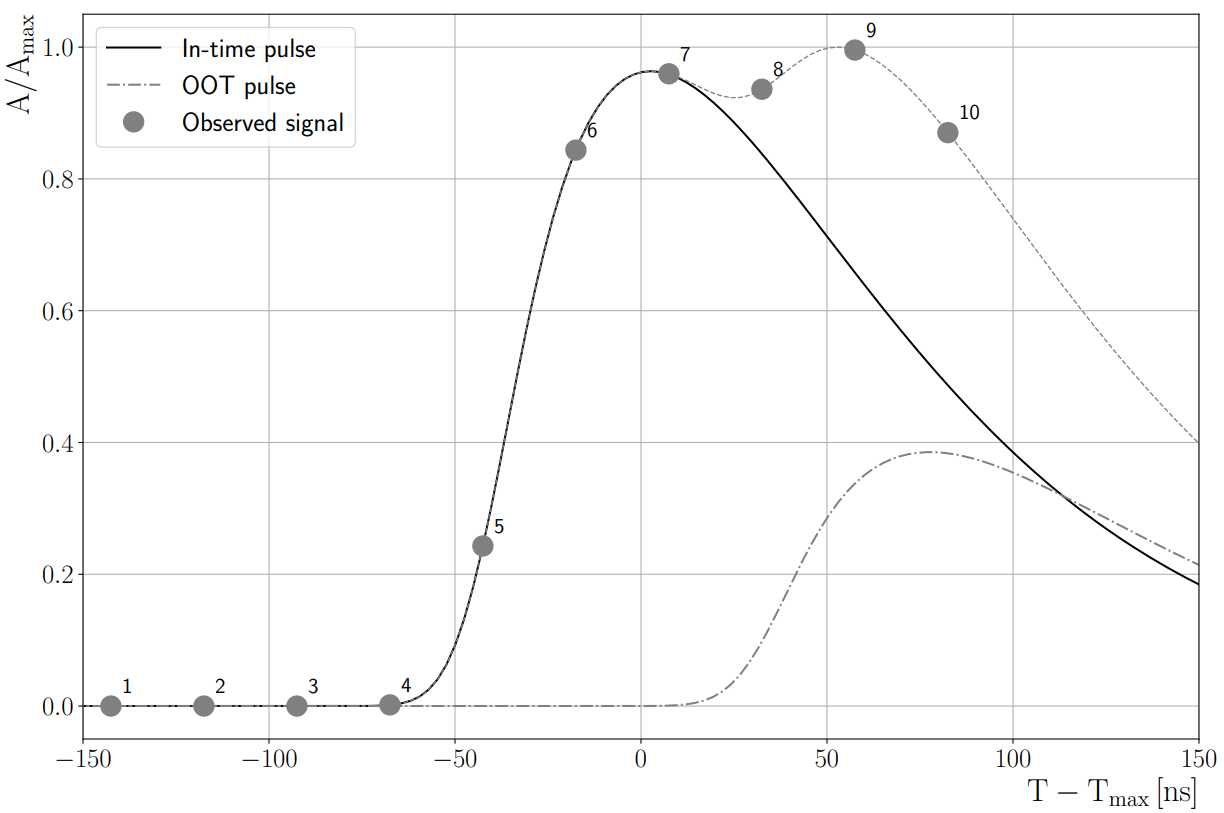
\includegraphics{fig/sec_reco/two_pulses.png}}
\caption{Example of a fitted ECAL pulse for a simulated event with an average of twenty pileup interactions and 25\,ns bunch spacing.
The measured pulse samples (points) are a superposition of an in-time pulse (solid line) and an out-of-time pulse (dashed line).
The amplitude is normalized to the maximum pulse amplitude $A_{\mathrm{max}}$, and the time axis is shown relative to the pulse maximum $T_{\mathrm{max}}$.}
\label{tec_multifit2}
\end{center}
\end{figure}

The ECAL time reconstruction developed for Run~I was used through the beginning of Run~III.
Owing to the fast scintillation response of PbWO$_4$ and the characteristics of the readout electronics, this method achieved time resolutions of order several hundred picoseconds for isolated interactions~\cite{Collaboration_2010}.
Residual channel-to-channel time offsets are corrected using calibration constants derived from data.
The resulting timing information is used, together with topological and energy-based criteria, to reject spurious signals inconsistent with energy deposits from particles produced in proton--proton collisions.
Such signals include direct ionization in the avalanche photodiodes (commonly referred to as spikes), as well as contributions from beam halo muons, cosmic rays, electronic noise, interactions in detector material, and OOT-PU~\cite{CMS-NOTE-2010-012}.

In the original implementation, the arrival time of a rechit was reconstructed by comparing the relative phases of the sampled pulse amplitudes to the expected pulse shape using ratios of consecutive samples.
While effective under the pileup conditions of Run~I, this ratio-based method does not fully account for the increased in-time and out-of-time pileup present in Run~II and Run~III.
The ratio-based time reconstruction algorithm and its limitations are discussed in Section~\ref{sec:algo1}.
To address these challenges, a new cross-correlation (CC) timing reconstruction method was developed during Run~II.
The CC algorithm and its performance are presented in Section~\ref{sec:algo2}.
%redone
\FloatBarrier
\subsection{Ratio Time Reconstruction \label{sec:algo1}}
%\subsection{Ratio Time Algorithm \label{sec:algo1}} 
As in the ECAL energy reconstruction, the ratio-based timing method estimates the time of a reconstructed hit (rechit) from the ten consecutively sampled pulse amplitudes recorded at 25\,ns intervals.
For an isolated signal with the expected pulse shape, the ratio of any two consecutive amplitude samples uniquely determines the relative timing of the pulse with respect to the LHC clock.
Figure~\ref{tec_pulseratio} shows the ratio
\[
R = \frac{A(T)}{A(T+25\,\mathrm{ns})}
\]
as a function of the time difference $T - T_{\mathrm{max}}$, where $T_{\mathrm{max}}$ denotes the time at which the pulse reaches its maximum amplitude.

The first three sampled amplitudes, $A(1)$, $A(2)$, and $A(3)$, are typically used to determine the pedestal value corresponding to zero signal and are therefore excluded from the timing reconstruction.
Ratios formed from $R\!\left(A(4)/A(5)\right)$ through $R\!\left(A(7)/A(8)\right)$ are used to estimate the pulse time.
Ratios involving samples on the falling tail of the pulse provide little sensitivity to the pulse timing and are not utilized.
The rechit time is determined from a weighted average of three consecutive ratio-based timing estimates derived from these sample pairs.

\begin{figure}[htbp]
\begin{center}
\resizebox{0.7\linewidth}{!}{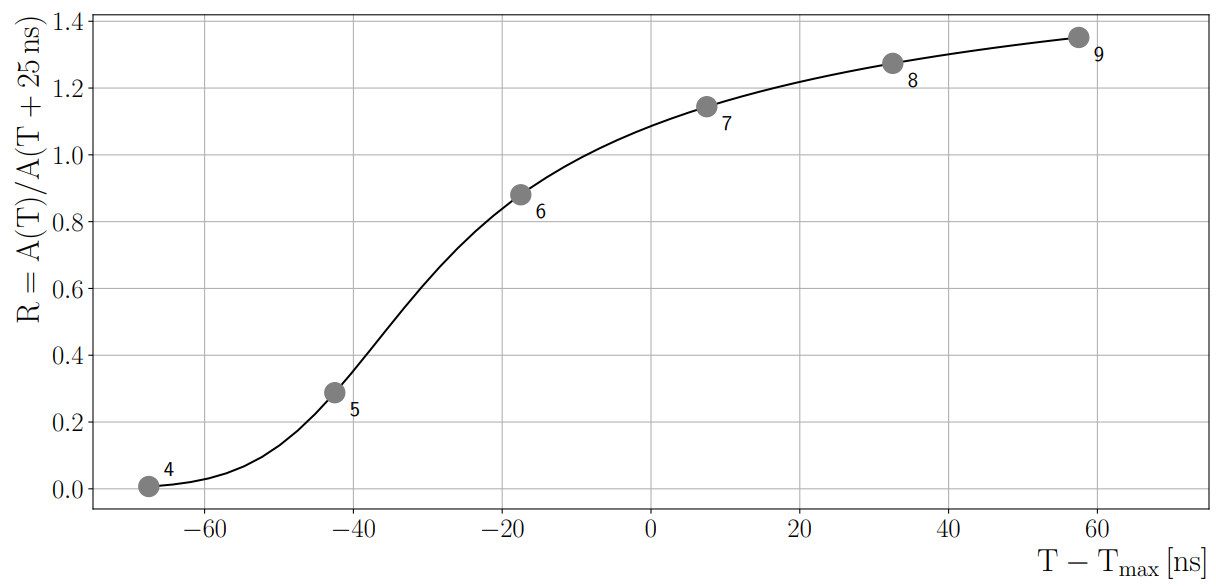
\includegraphics{fig/sec_reco/ratio_tvR_mod.png}}
\caption{Ratio $R$ of two consecutive pulse amplitudes, $A(T)$ and $A(T+25\,\mathrm{ns})$, as a function of the time difference $T - T_{\mathrm{max}}$.
The first three samples, $A(1)$--$A(3)$, which are used for pedestal determination, are excluded.
The rechit time is obtained from a weighted average of the timing estimates derived from the ratios $R\!\left(A(4)/A(5)\right)$ through $R\!\left(A(7)/A(8)\right)$.}
\label{tec_pulseratio}
\end{center}
\end{figure}

Channel-dependent delays in the clock distribution system introduce offsets between the reconstructed pulse time and the true particle arrival time.
These offsets vary from crystal to crystal and are corrected using calibration constants derived from prompt relativistic particles, such that the mean reconstructed time for each channel is centered at zero~\cite{CMS-PAS-EXO-19-005}.

The time of arrival of a reconstructed particle at the ECAL, $t_{\mathrm{ECAL}}$, is computed as a weighted average of the rechit times from the individual crystals comprising the associated ECAL cluster,
\begin{equation}
t_{\mathrm{ECAL}} =
\frac{\sum_{i} t^{i}_{\mathrm{ECAL}} / \sigma^{2}_{i}}
     {\sum_{i} 1 / \sigma^{2}_{i}} \, ,
\label{ratio_eqt}
\end{equation}
where $t^{i}_{\mathrm{ECAL}}$ is the reconstructed time of the rechit in crystal $i$ and $\sigma_{i}$ is the estimated time resolution for that crystal.
The resolution weights $\sigma_{i}$ are derived from the intrinsic timing performance of the ECAL crystal and readout system~\cite{Collaboration_2010}.

The ratio-based timing method assumes that the sampled signal pulse is well isolated in time.
In the higher pileup environments of Run~II and Run~III, this assumption is no longer valid.
As discussed previously, the observed pulse shape in an ECAL channel is generally a superposition of an in-time pulse and multiple non-negligible out-of-time contributions arising from pileup and out-of-time pileup (OOT-PU).
In such cases, the sampled pulse shape deviates significantly from the nominal pulse template.
When this occurs, the ratio of two consecutive samples no longer provides a unique mapping to the pulse time, resulting in degraded timing resolution and increased sensitivity to pileup-induced biases.
%redone
\FloatBarrier
\subsection{Cross Correlation Time Algorithm \label{sec:algo2}}
The degradation of ECAL timing performance in the presence of out-of-time pileup motivates the development of a timing reconstruction method that explicitly accounts for overlapping pulses.
To address this, a cross-correlation (CC) timing algorithm has been developed that exploits the pulse amplitudes reconstructed by the multi-fit energy reconstruction.

The CC method uses the ten fitted pulse amplitudes, $A^{\mathrm{mf}}_{i}$, obtained from the multi-fit algorithm.
The measured pulse shape in a given crystal, denoted $H(\mathrm{BX})$, can be expressed as a linear superposition of contributions from the nominal in-time pulse and up to nine out-of-time (OOT) pulses originating from pileup interactions in neighboring bunch crossings.
Each of these contributions arises from scintillation light produced by particles incident in the crystal and is therefore expected to follow the same characteristic pulse shape.
While the amplitudes of these contributions are reconstructed by the multi-fit algorithm, the precise timing offset of each pulse relative to the nominal interaction is not known \emph{a priori}.

\begin{figure}[htbp]
\begin{center}
\resizebox{0.95\linewidth}{!}{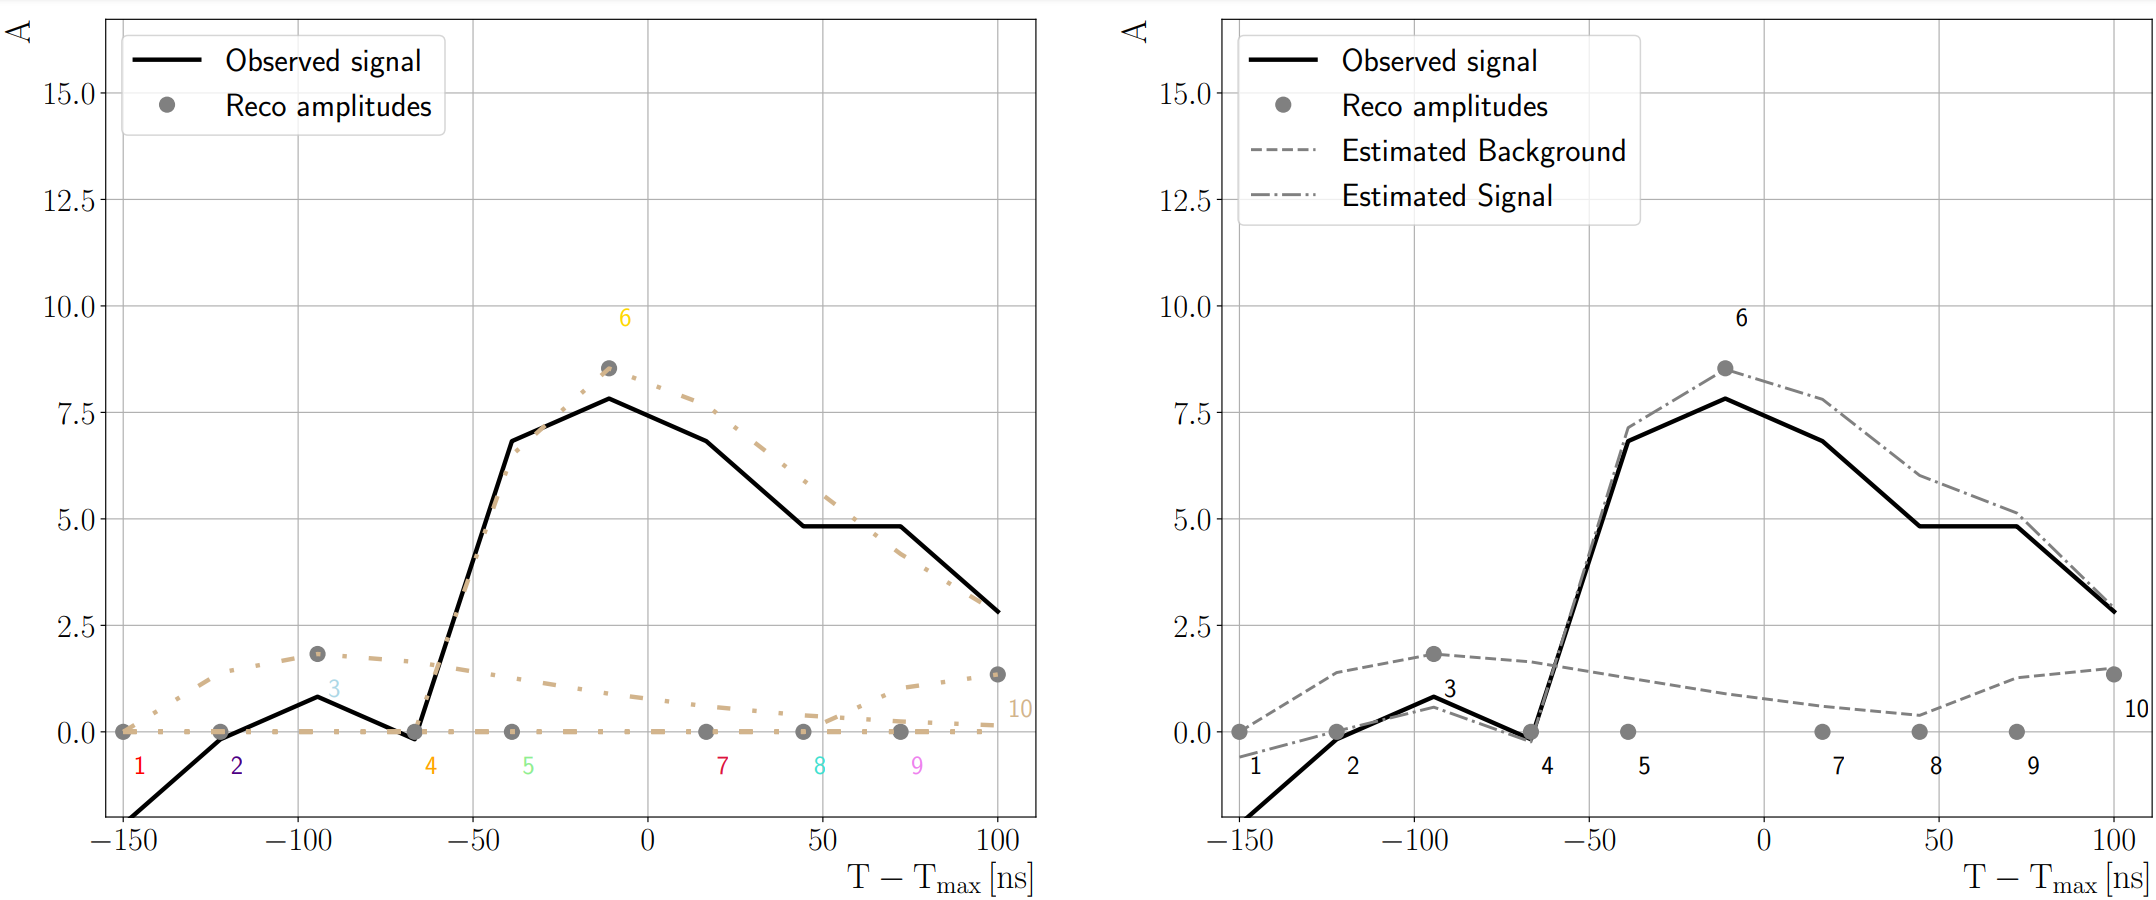
\includegraphics{fig/sec_algos/fOOT_reco_a2.png}}
\caption{Illustration of the OOT amplitude correction procedure used in the CC timing reconstruction.
In both panels, the solid black line shows the measured pulse shape $H(\mathrm{BX})$, and the black points indicate the fitted multi-fit amplitudes $A^{\mathrm{mf}}_{i}$.
Left: the reconstructed in-time and out-of-time pulse contributions $F^{\mathrm{OOT}}_{i}(A^{\mathrm{mf}}_{i},t)$.
Right: the background pulse shape $F_{\mathrm{bg}}(\mathrm{BX},t)$ obtained from the superposition of OOT contributions (dash-dotted line) and the recovered in-time signal $A^{\mathrm{sig}}(\mathrm{BX},t)$ after subtraction (dashed line).}
\label{tra_pulsereco}
\end{center}
\end{figure}

To enable continuous time shifts of the pulse shape, an analytic description of the characteristic ECAL pulse shape is constructed by fitting a parameterized function to the measured pulse templates on a channel-by-channel basis.
Using this analytic representation together with the fitted amplitudes $A^{\mathrm{mf}}_{i}$, a function
$F^{\mathrm{OOT}}_{i}(A^{\mathrm{mf}}_{i},t)$
is defined to describe the amplitude and time dependence of each OOT pulse contribution.
The total OOT background pulse shape is then obtained as the linear superposition
\begin{equation}
F_{\mathrm{bg}}(\mathrm{BX},t) =
\sum_{i} F^{\mathrm{OOT}}_{i}(A^{\mathrm{mf}}_{i},t) \, ,
\label{cc_bps}
\end{equation}
where the sum runs over all reconstructed OOT contributions.

The in-time signal pulse is recovered by subtracting the OOT background from the measured pulse shape,
\begin{equation}
A^{\mathrm{sig}}(\mathrm{BX},t) =
H(\mathrm{BX}) - F_{\mathrm{bg}}(\mathrm{BX},t) \, .
\label{cc_sig}
\end{equation}
If the correct timing parameters are used in the construction of $F^{\mathrm{OOT}}_{i}$, the recovered signal $A^{\mathrm{sig}}(\mathrm{BX},t)$ follows the expected characteristic pulse shape of an isolated scintillation signal.
This procedure is referred to as the \emph{OOT amplitude correction}.

The second step of the CC algorithm determines the arrival time of the in-time pulse by matching $A^{\mathrm{sig}}(\mathrm{BX},t)$ to the pulse shape template $S[\mathrm{BX}]$.
A normalized cross-correlation function is constructed,
\begin{equation}
d(\delta) \equiv
\frac{\sum_{\mathrm{BX}} A^{\mathrm{sig}}(\mathrm{BX},t)\,S(\mathrm{BX},\delta)}
     {\sqrt{\sum_{\mathrm{BX}} \left(A^{\mathrm{sig}}(\mathrm{BX},t)\right)^{2}}
      \sqrt{\sum_{\mathrm{BX}} \left(S(\mathrm{BX},\delta)\right)^{2}}} \, ,
\label{cc_delta}
\end{equation}
where $S(\mathrm{BX},\delta)$ denotes the pulse template shifted by a time offset $\delta$.
The reconstructed rechit time corresponds to the value of $\delta$ that maximizes the cross-correlation function $d(\delta)$.
This procedure is referred to as the \emph{cross-correlation fit}.

For reconstructed pulses with delays exceeding approximately 1\,ns, the OOT amplitude correction exhibits a systematic bias that leads to an underestimation of the reconstructed time.
This effect, and its impact on delayed signals, is discussed in detail in Section~\ref{sec:recobias}.
 %redone
%\subsubsection{Slew Issue Correction \label{sec:algo21}}
%This is some text on slew issue correction.

%\FloatBarrier
\subsubsection{Delay Time Bias \label{sec:recobias}}
The majority of physics analyses that employ ECAL timing focus on prompt signals, defined as energy deposits arising from particles produced at the primary vertex (PV) with no significant displacement in space or delay in time.
In contrast, delayed signals arise when a long-lived particle (LLP) travels a macroscopic distance from the PV before decaying, often with a velocity $\beta < 1$.
The decay products of such particles can therefore arrive at the ECAL with significantly delayed times relative to prompt particles.
Accurate reconstruction of large delay times is essential for analyses targeting LLP signatures.

The performance of the CC timing algorithm for delayed signals is studied using simulated samples containing LLP decays that produce sizable delays in the ECAL.
To quantify the accuracy of the reconstructed times, a reference generator-level time is required.
For each reconstructed hit (rechit), a generator-level time (\emph{gen-time}) is computed from the simulated energy deposits in the ECAL crystals, recorded as \texttt{pCaloHits}.
The gen-time of a rechit is defined as the energy-weighted average of the times of the \texttt{pCaloHits} contributing to the reconstructed pulse.

Figure~\ref{pc_v_cc_bais} shows the reconstructed rechit time obtained with the CC algorithm as a function of the corresponding gen-time.
No timing calibration is applied to the reconstructed times.
For delays exceeding approximately 1~ns, a systematic bias is observed, with the reconstructed time underestimating the true delay.
The right panel of Fig.~\ref{pc_v_cc_bais} shows an expanded view of the region below approximately 1~ns, where good agreement between the CC reconstruction and the gen-time is observed, indicating accurate performance for prompt and mildly delayed signals.

\begin{figure}[h!tbp]
\begin{center}
\resizebox{0.45\textwidth}{!}{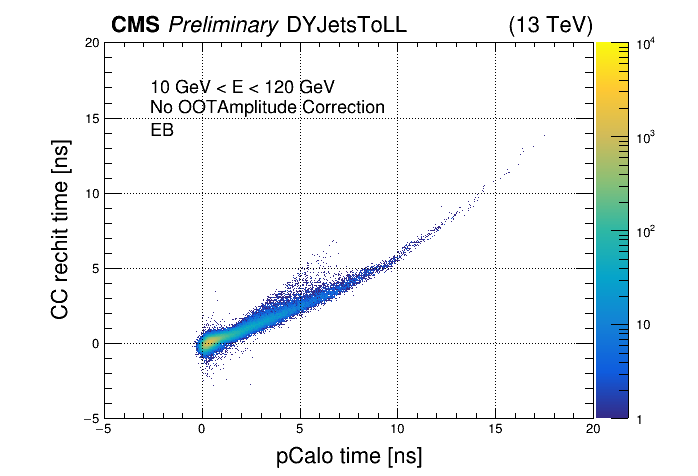
\includegraphics{fig/sec_gen/tr_2d_PCvCC_delay_13062022150058.png}}
\resizebox{0.45\textwidth}{!}{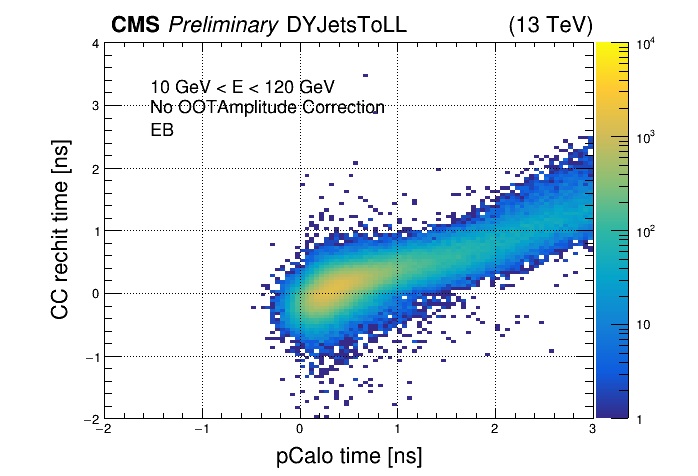
\includegraphics{fig/sec_gen/tr_2d_PCvCC_delay_zoom_13062022150920.png}}
\caption{Generator-level rechit time as a function of the rechit time reconstructed with the CC algorithm in simulated events containing delayed signals.
The reconstructed times are uncalibrated.
Left: a systematic bias is observed for delays greater than approximately 1~ns.
Right: an expanded view of the region below approximately 1~ns, where good agreement with the generator-level time is observed.}
\label{pc_v_cc_bais}
\end{center}
\end{figure}

To identify the origin of this bias, the CC timing reconstruction is repeated with the out-of-time (OOT) amplitude correction disabled.
Figure~\ref{pc_v_cc_nooot} shows the reconstructed rechit time obtained with this modified CC algorithm as a function of the gen-time.
In this configuration, no significant bias is observed at large delay times, demonstrating that the bias originates from the OOT amplitude correction step.

\begin{figure}[h!tbp]
\begin{center}
\resizebox{0.7\textwidth}{!}{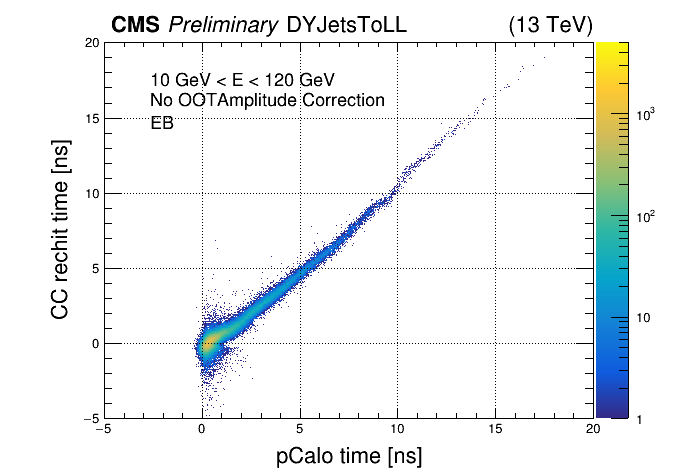
\includegraphics{fig/sec_gen/tr_2d_PCvCC_delay_nocorr_09062022175333.png}}
\caption{Generator-level rechit time as a function of the rechit time reconstructed with the CC algorithm when the OOT amplitude correction is disabled.
No significant bias is observed at large delay times.}
\label{pc_v_cc_nooot}
\end{center}
\end{figure}

As discussed in Section~\ref{sec:algo2}, the OOT amplitude correction relies on amplitudes returned by the multi-fit energy reconstruction, which assumes that out-of-time contributions occur at fixed time offsets corresponding to integer multiples of the LHC bunch spacing.
For delayed signals, this assumption is violated because the relative timing of pulse contributions varies continuously with the particle time of flight.
As a result, the fitted OOT amplitudes no longer accurately describe the true pulse composition, leading to a biased correction of the reconstructed pulse shape and, consequently, of the reconstructed time.

To accommodate analyses involving delayed signatures, the CC algorithm provides two reconstructed time quantities: one with and one without the OOT amplitude correction.
The corrected time, which benefits from mitigation of OOT pileup, is optimal for prompt physics analyses.
The uncorrected time, while exhibiting degraded resolution due to residual pileup contributions, remains unbiased at large delays and is therefore suitable for analyses targeting LLP signatures.
Both timing quantities are available in the ECAL reconstructed hit collection within the CMS software framework (CMSSW).
%redone
\FloatBarrier
\subsubsection{Spike Rejection Parameters \label{sec:resspkdata} }
Anomalous isolated energy deposits with reconstructed energies that can exceed 100~GeV have been observed in the ECAL.
These deposits, commonly referred to as \emph{spikes}, occur at a rate proportional to the collision rate and can create significant challenges for triggering at high luminosity.
If not rejected, spikes can bias the reconstructed energies and times of electrons, photons, jets, and the missing transverse momentum in an event.
In the ECAL barrel, spikes originate primarily from particles directly striking the avalanche photodiodes (APDs), producing large signals through direct ionization in the silicon sensor~\cite{Petyt:2012upa}.
Spike energy is typically concentrated in a single crystal and is characterized by a fast-rising pulse shape with little or no scintillation component.
In most cases there is minimal activity in neighboring crystals, although occasional ``double spikes'' produce spike-like signals in two adjacent crystals.
A reconstructed hit (rechit) produced by a spike is referred to as a \emph{spike rechit}.

The performance of standard spike-rejection flags is studied in the context of the CC timing reconstruction.
For this study, rechit collections are produced for both the ratio and CC timing methods and stored directly as output of the corresponding reconstruction modules, without downstream cleaning, filtering, or timing calibration.
The CC reconstruction is performed without the OOT amplitude correction to minimize time-dependent effects arising from the energy reconstruction.
These collections are referred to as \emph{raw} rechit collections.

\begin{figure}[h!tbp]
\begin{center}
\resizebox{0.75\textwidth}{!}{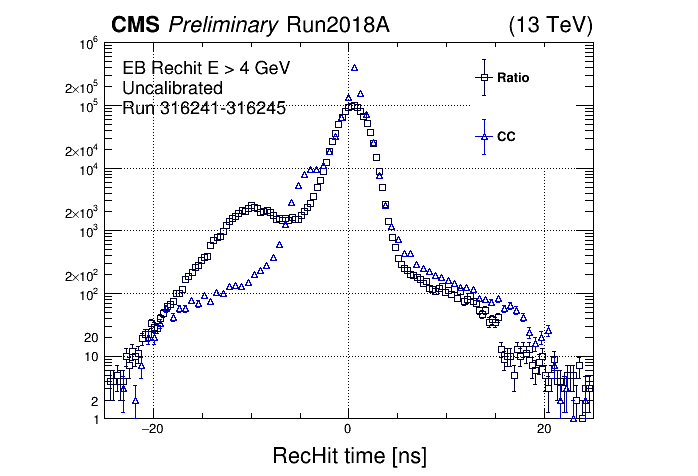
\includegraphics{fig/sec_gen/tr_hl_spike_distro_10062022142744.png}}
\caption{Distribution of rechit times reconstructed with the ratio method and the CC method for rechits with energy $>4$~GeV, using raw rechit collections saved without downstream cleaning, filtering, or calibration.
Secondary structures at approximately $-10$~ns (ratio) and $-5$~ns (CC) are dominated by spike rechits.}
\label{raw_distro}
\end{center}
\end{figure}

Figure~\ref{raw_distro} shows the rechit time distributions in the raw collections for rechits with energy greater than 4~GeV.
Secondary structures are observed at approximately $-10$~ns for the ratio method and $-5$~ns for the CC method; these features are dominated by spike rechits.
Figure~\ref{2d_raw_distro_comp} shows the correlation between the raw CC and ratio rechit times for rechits with energies between 10 and 120~GeV.
A strong correlation is observed between the reconstructed times obtained with the two methods, while the CC method exhibits a narrower prompt-time population.
In this sample, spike rechits populate an early-time region spanning approximately $-6$ to $-15$~ns for the ratio method and $-2$ to $-10$~ns for the CC method.

\begin{figure}[h!tbp]
\begin{center}
\resizebox{0.7\textwidth}{!}{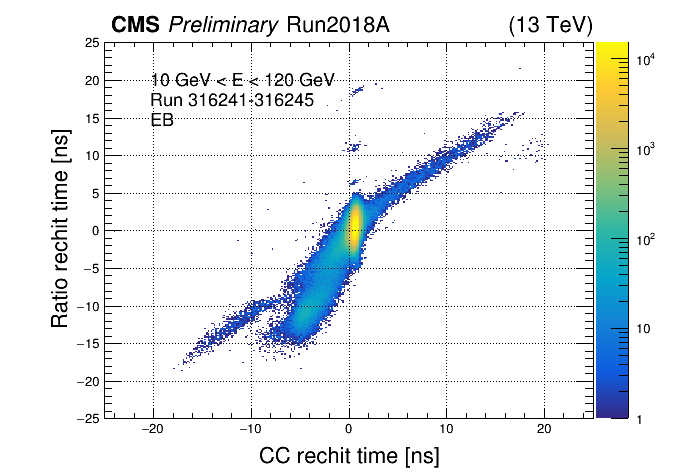
\includegraphics{fig/sec_gen/tr_2d_RtvCC_spike_10062022125336.png}}
\caption{Correlation of raw rechit times reconstructed with the CC method and the ratio method for rechits with energies between 10 and 120~GeV.
The CC method exhibits a narrower prompt-time population.
Spike rechits populate an early-time region at approximately $-6$ to $-15$~ns for the ratio method and $-2$ to $-10$~ns for the CC method.}
\label{2d_raw_distro_comp}
\end{center}
\end{figure}

Spike rechits are characterized by reconstructed times that are significantly earlier than those of scintillation-induced signals.
For spike-like pulse shapes, the fast rise time biases the ratio-based timing reconstruction toward earlier times.
The CC method is less sensitive to this effect and yields a smaller, though still non-negligible, early-time bias.
In addition, spike rechits are typically isolated from surrounding activity.
Since isolated high-energy deposits are inconsistent with electromagnetic shower development, spike rejection can exploit both the topology of local energy sharing and the reconstructed time.

The swiss-cross variable characterizes the degree of energy sharing between a crystal with a large deposit and its nearest neighbors, with values closer to one indicating a more isolated deposit.
The swiss-cross is used to define topological spike-rejection flags, including \texttt{kWeird}, which rejects isolated energy deposits, and \texttt{kDiWeird}, which targets double spikes~\cite{Petyt:2012upa}.
In addition, a timing-based rechit flag \texttt{kOutOfTime} (\texttt{kOOT}) is defined using energy-dependent time thresholds that may be configured separately for the barrel and endcaps and for different energy ranges.
This flag defines a time window around the prompt population and marks rechits reconstructed outside this window on either the early or delayed side.

\begin{figure}[h!tbp]
\begin{center}
\resizebox{0.375\textwidth}{!}{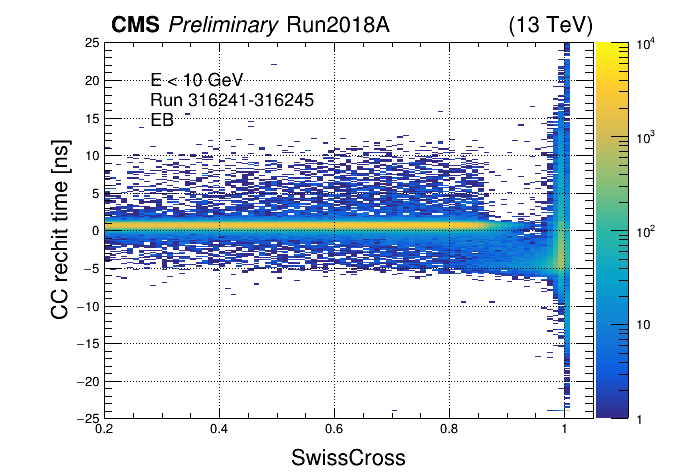
\includegraphics{fig/sec_gen/tr_2d_CC_swisscross1_10062022134628.png}}
\resizebox{0.375\textwidth}{!}{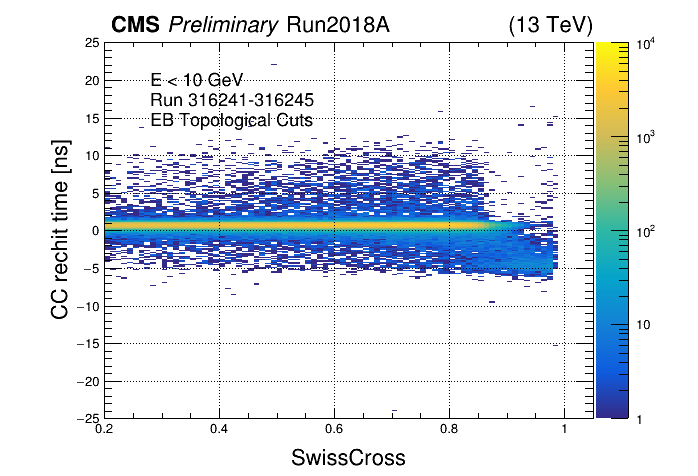
\includegraphics{fig/sec_gen/tr_2d_CC_swisscross2_10062022134846.png}}
\resizebox{0.375\textwidth}{!}{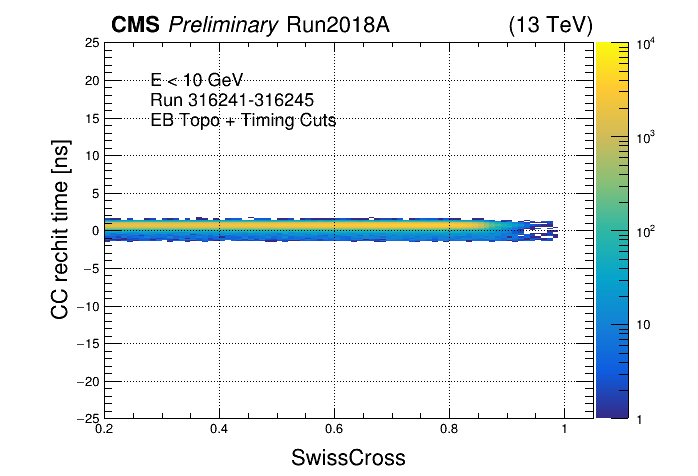
\includegraphics{fig/sec_gen/tr_2d_CC_swisscross3_10062022135015.png}}
\caption{Swiss-cross as a function of CC reconstructed rechit time for rechits with energy $>10$~GeV.
Left: distribution without spike-rejection cuts, showing a prompt population and a spike-dominated population at large swiss-cross values and early reconstructed times.
Middle: distribution after applying the topological spike-rejection flags (\texttt{kWeird} and \texttt{kDiWeird}), where most spike rechits are removed, though a residual early-time feature remains.
Right: distribution after additionally applying the \texttt{kOOT} timing flag using a 3~ns threshold for all timing parameters, where the remaining spike population is strongly suppressed.}
\label{swisscross_CC}
\end{center}
\end{figure}

A rechit flagged as \texttt{kOOT} is unlikely to be used in downstream particle reconstruction, and overly aggressive timing thresholds can therefore reduce the reconstructed energy of physics objects.
It is consequently necessary to tune the \texttt{kOOT} thresholds for the CC time reconstruction to maximize spike rejection while minimizing impact on prompt scintillation signals across the full rechit energy range.
Since CC reconstructed times exhibit a different energy dependence than ratio reconstructed times, the optimal \texttt{kOOT} parameter values for low- and high-energy rechits must be determined independently.

Based on these studies, the \texttt{kOOT} timing thresholds for the CC reconstruction are tuned to achieve efficient rejection of spike rechits while preserving prompt scintillation signals across the full rechit energy range.
Separate threshold values are optimized for low- and high-energy rechits to account for the energy dependence of the CC reconstructed time.
The selected parameter configuration provides strong suppression of spike-induced early-time populations with minimal impact on downstream particle reconstruction.
Unless otherwise stated, this tuned \texttt{kOOT} configuration is used for the CC timing reconstruction in all subsequent performance studies presented in this paper.
%redone
%\FloatBarrier
%\subsection{Sensitivity of time reconstruction at delayed times to out-of-time amplitudes \label{sec:reslldata} }
%\subsubsection{Truth Times \label{sec:resmeth2}}
%Resolution studies characterize the precision of a timing reconstruction method but do not measure the accuracy of the reconstruction. It is possible to achieve a very precise result, and therefore an objectively good time resolution, by arbitrarily setting the reconstructed time of all rechits to a constant value with some random jitter. In order to test the accuracy of the reconstruction methods, the ability to compare the results of the reconstructed rechit time to a true time for that rechit is required. This is typically done with Monte-Carlo (MC) truth information. Unfortunately such information, while in development, is not available in current MC datasets.

\hfill
\begin{figure}[htbp]
\begin{center}
\resizebox{0.32\textwidth}{!}{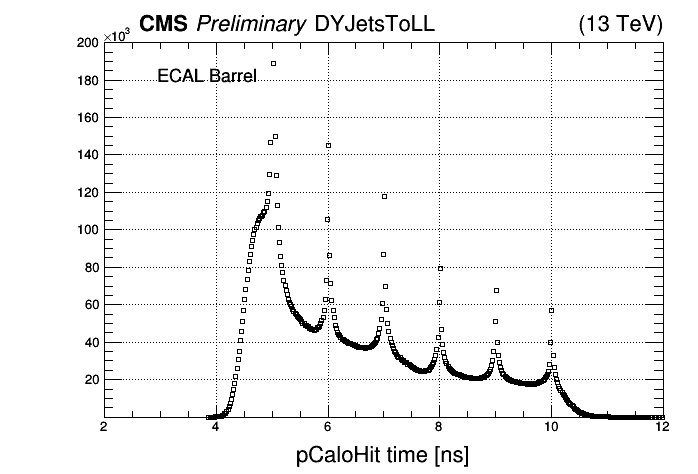
\includegraphics{fig/sec_gen/tr_pcalo_time_hit_18112020145605.png}}
\resizebox{0.32\textwidth}{!}{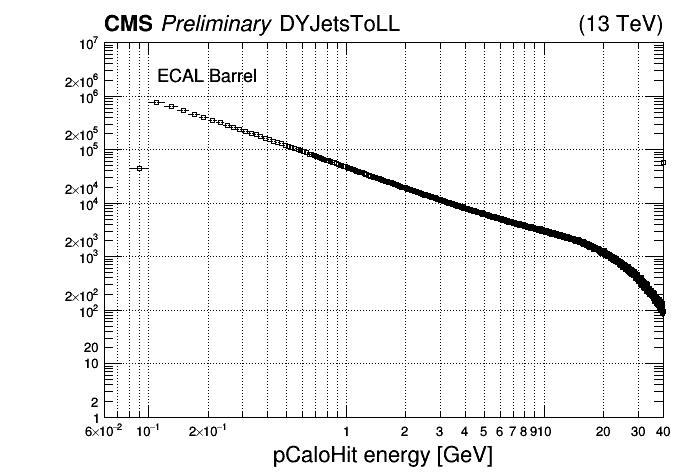
\includegraphics{fig/sec_gen/tr_pcalo_energy_hit_18112020150843.png}}
\resizebox{0.32\textwidth}{!}{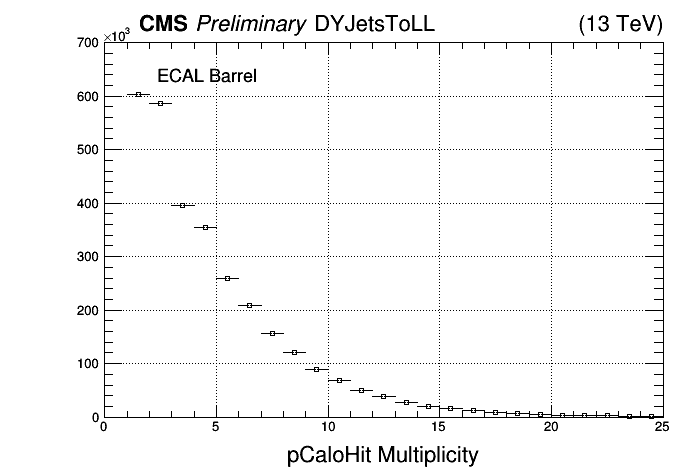
\includegraphics{fig/sec_gen/tr_pcalo_phomulti_hist_25112020111944.png}}
\caption{Time (left), energy (middle), and multiplicity (right) distributions of the pCaloHit information recorded in the pCaloHit collection.} 
\label{pc_etm}
\end{center}
\end{figure} 

In order to formulate a reference time, or \emph{gen time}, with existing MC that can be compared, rechit by rechit, with the reconstructed time, the information in the pCaloHit collection was utilized. The pCaloHit collection records the simulated deposition of energy in a crystal during an event and the time, relative to the bunch crossing, at which this energy was deposited in the crystal. Shower and event development may result in multiple energy depositions in a single crystal and at various depths within the crystal. A single pCaloHit is generated for each of the multiple energy depositions in a crystal. Unfortunately, while variables to record the depth information are present in the pCaloHit collection, in current simulation this information is not recorded by default. 

As can be seen in Figure~\ref{pc_etm} from the distributions of the time, energy, and multiplicity distributions of pCaloHit hits, the pCaloHit times are produced in smeared intervals from approximately five to ten nanoseconds, which is consistent with time of flight from the CMS origin to the physical location of the crystals. The pCaloHit times do not account for variations in the location of the interaction on the crystal face or the resolution of the location of the primary vertex. The energy and multiplicity distributions show that there are typically multiple pCaloHits in a crystal for any interaction and that these hits are produced with a uniform distribution of energy to be deposited in the crystals.

\hfill
\begin{figure}[htbp]
\begin{center}
\resizebox{0.7\textwidth}{!}{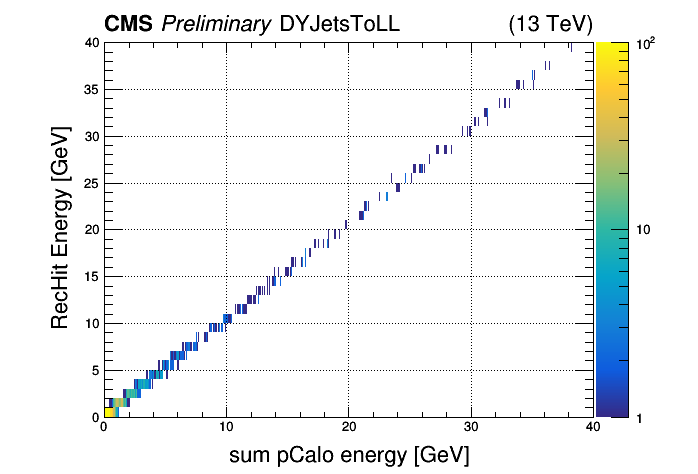
\includegraphics{fig/sec_gen/tr_2d_pce_v_rhe_12112020160129.png}}
\caption{Sum of the pCaloHit energies for pCaloHits geometrically matched to a single crystal correlated with the rechit energy for the rechit that corresponds to that crystal.}
\label{pc_evrhe}
\end{center}
\end{figure}

In order to reconstruct a gen time reference, the pCaloHits are geometrically matched to the crystals in which those hits occur. A collection of pCaloHits for a specific crystal that corresponds to the rechit in that crystal is thereby obtained. In order to validate that this selection of the pCaloHits in a crystal is matched to a specific rechit, the sum of the energies of the selected pCaloHits are compared to the corresponding rechit energy. As can be seen in Figure~\ref{pc_evrhe}, the sum of the pCaloHit energies has a roughly one to one correlation with the rechit energy. This was studied using the g4SimHits, Mix, pCaloHit collection in :
\begin{center}
DYJetsToLL\_M-50\_TuneCP5\_13TeV-madgraphMLM- pythia8 
RunIIAutumn18MiniAODFlatPU28to62NZS\_102X\_upgrade2018\_realistic\_v15-v1 
\end{center}
%in MINIAODSIM and GEN-SIM-RAW with CMSSW 10.2.5 and GT: 102X\_upgrade2018\_realistic\_v20. 

\begin{figure}[htbp]
\begin{center}
\subfloat[pCaloHit time in the four separate crystals studied. ]{
\resizebox{0.24\textwidth}{!}{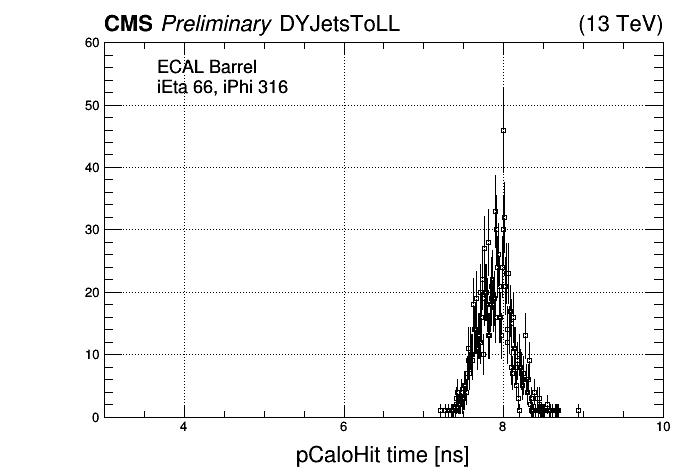
\includegraphics{fig/sec_gen/tr_pcaloMtime0_hist_23112020160113.png}}
\resizebox{0.24\textwidth}{!}{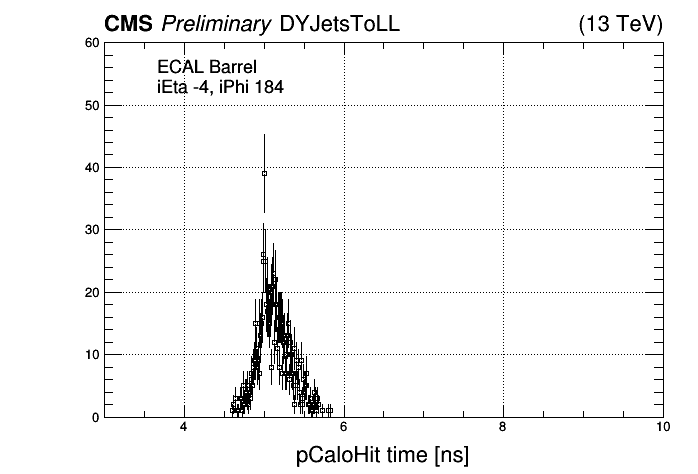
\includegraphics{fig/sec_gen/tr_pcaloMtime1_hist_23112020160311.png}}
\resizebox{0.24\textwidth}{!}{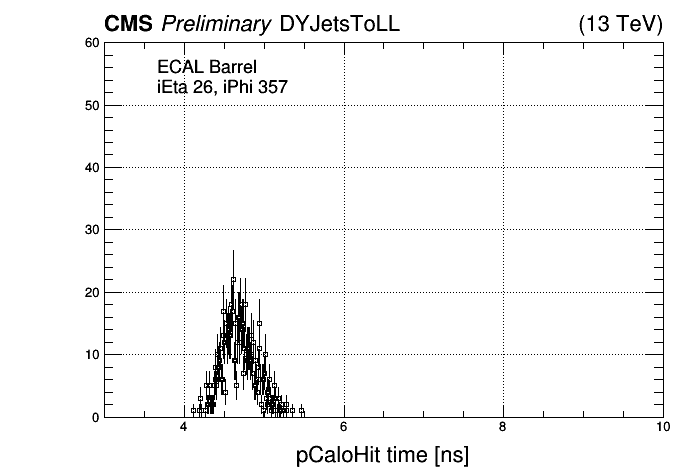
\includegraphics{fig/sec_gen/tr_pcaloMtime2_hist_23112020160510.png}}
\resizebox{0.24\textwidth}{!}{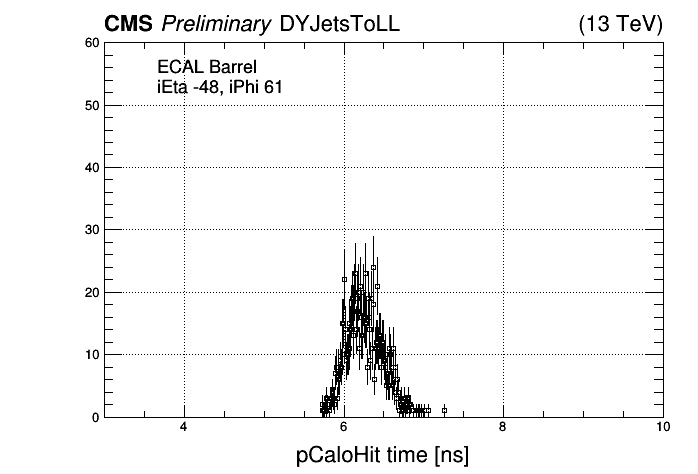
\includegraphics{fig/sec_gen/tr_pcaloMtime3_hist_23112020160828.png}}
\label{pc_4c_pct}}

\subfloat[pCaloHit multiplicity in the four separate crystals studied. ]{
\resizebox{0.24\textwidth}{!}{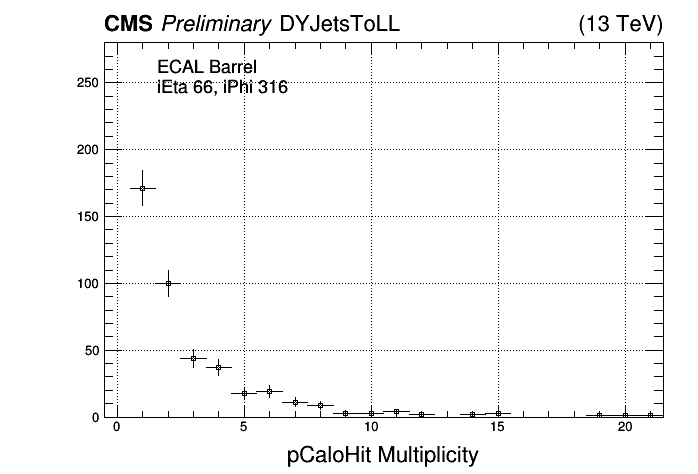
\includegraphics{fig/sec_gen/tr_pcaloMulti0_hist_23112020164218.png}}
\resizebox{0.24\textwidth}{!}{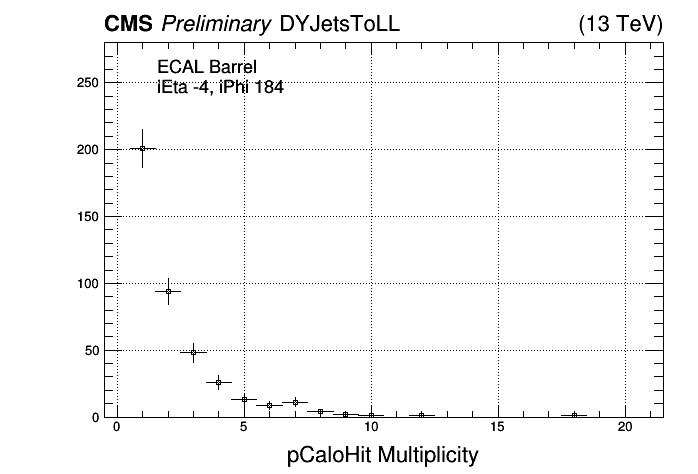
\includegraphics{fig/sec_gen/tr_pcaloMulti1_hist_23112020164317.png}}
\resizebox{0.24\textwidth}{!}{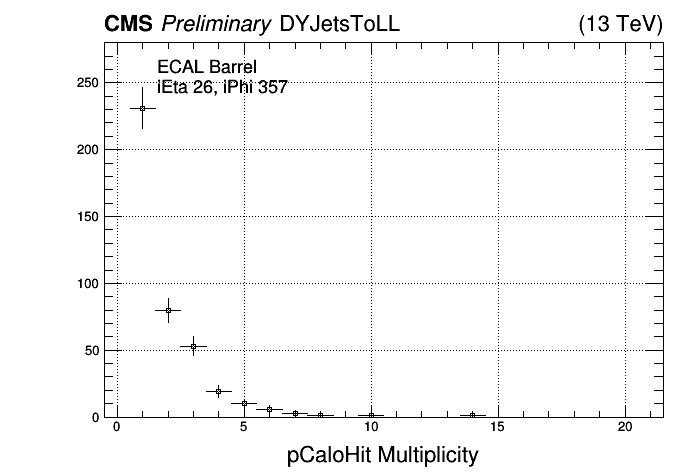
\includegraphics{fig/sec_gen/tr_pcaloMulti2_hist_23112020164503.png}}
\resizebox{0.24\textwidth}{!}{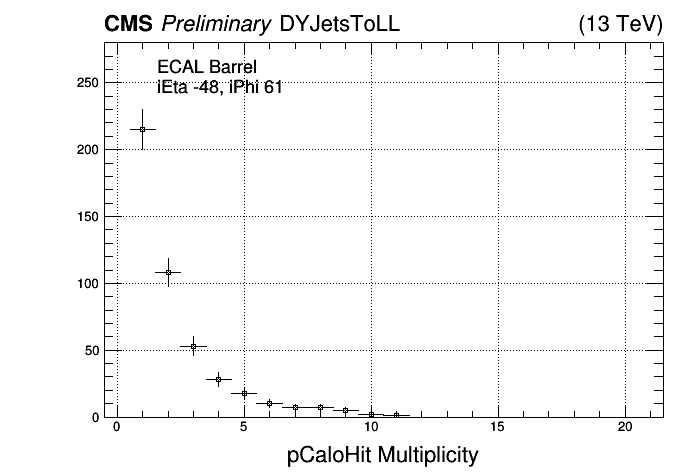
\includegraphics{fig/sec_gen/tr_pcaloMulti3_hist_23112020164600.png}}
%\caption{pCaloHit multiplicity in the four separate crystals studied. } 
\label{pc_4c_pcm}}

\subfloat[Weighted RMS of pCaloHit time in the four separate crystals studied. ]{
\resizebox{0.24\textwidth}{!}{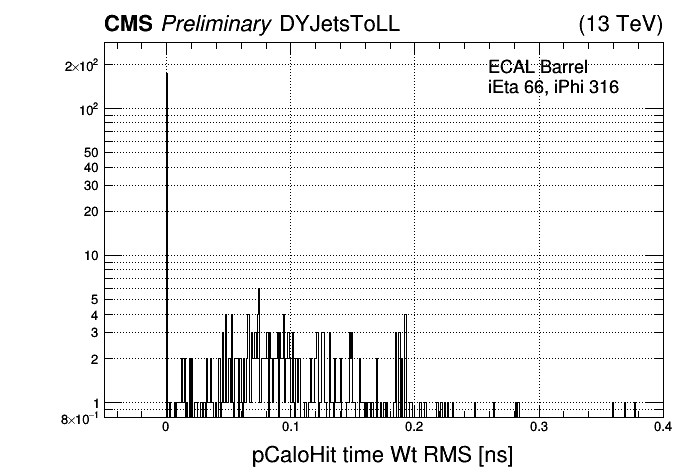
\includegraphics{fig/sec_gen/tr_pcaloWtRMS0_hist_23112020165226.png}}
\resizebox{0.24\textwidth}{!}{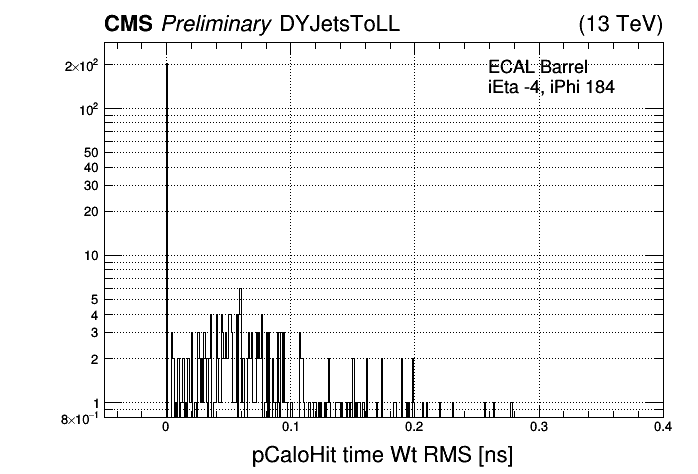
\includegraphics{fig/sec_gen/tr_pcaloWtRMS1_hist_23112020165419.png}}
\resizebox{0.24\textwidth}{!}{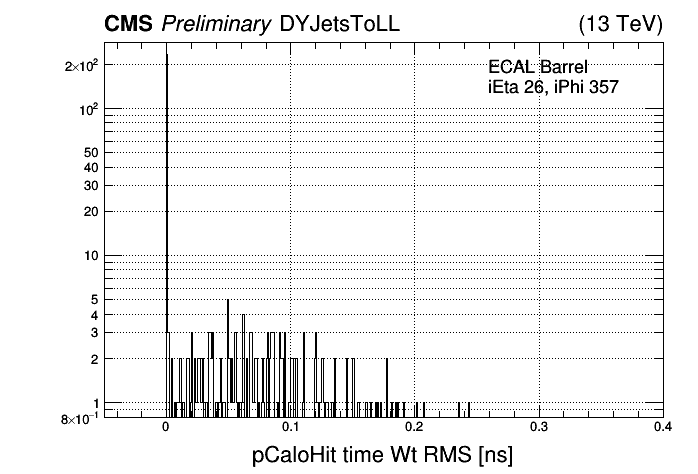
\includegraphics{fig/sec_gen/tr_pcaloWtRMS2_hist_23112020165539.png}}
\resizebox{0.24\textwidth}{!}{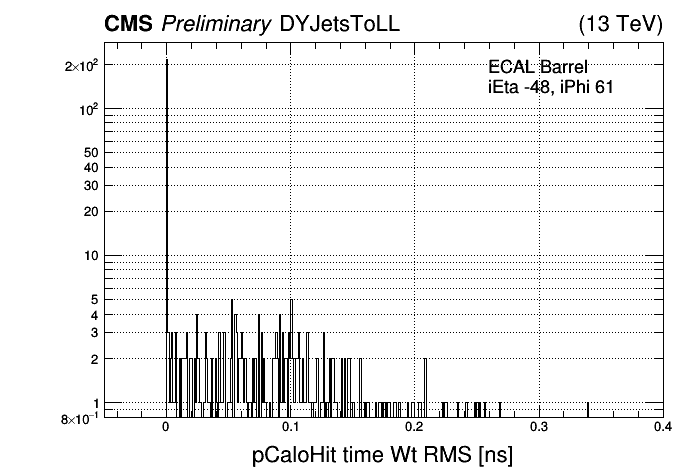
\includegraphics{fig/sec_gen/tr_pcaloWtRMS3_hist_23112020165750.png}}
\label{pc_4c_rms}}
\caption{pCaloHit time distribution, multiplicity, and Wt. RMS of the time for pCaloHits geometrically matched to four separate crystals in ECAL Barrel. These crystals are located, from left to right, at (ieta, iphi) of : (66,316), (26,357), (-4,184), and (-48,61) in the EB. Note that in the Wt. RMS plots the spike at zero correspond to crystal with a single pCaloHit.}
\label{pc_4c_all}
\end{center}
\end{figure} 

These collections of pCaloHits geometrically matched to a single crystal were studied in four randomly selected crystals spread along the ECAL barrel in eta and phi. From the matched pCaloHits in these crystals the energy weighted RMS of the pCaloHit times was determined. In Figure~\ref{pc_4c_all} of the pCaloHit times, multiplicity, and the Wt. RMS of the times in these four crystals are shown. It can be seen that while the mean value the time distributions varies according to the time of flight distance for each of the specific crystals, the distribution of these values are roughly the same in all four crystals with a spread in the times under one nanosecond. In Figure~\ref{pc_rms} the event by event Wt. RMS for the pCaloHit times in all barrel crystals is shown. It can be seen that the Wt. RMS of the pCaloHits, in crystals with a multiplicity greater than one, peaks at $\sim$60-80 ps.

\begin{figure}[htbp]
\begin{center}
%\resizebox{0.48\textwidth}{!}{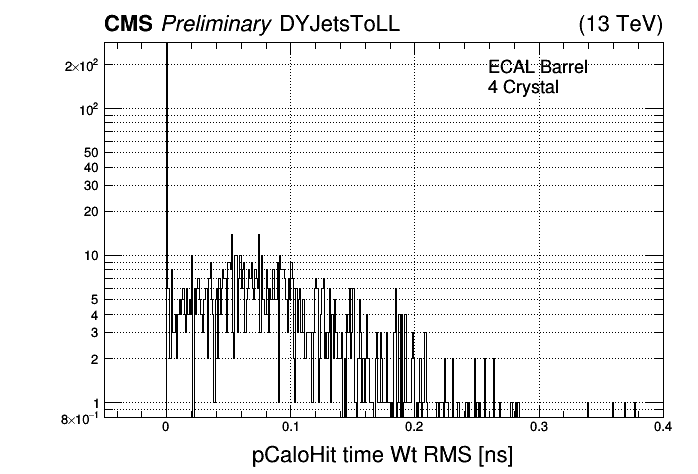
\includegraphics{fig/sec_gen/tr_pcaloWtRMS_hist_23112020165948.png}}
\resizebox{0.7\textwidth}{!}{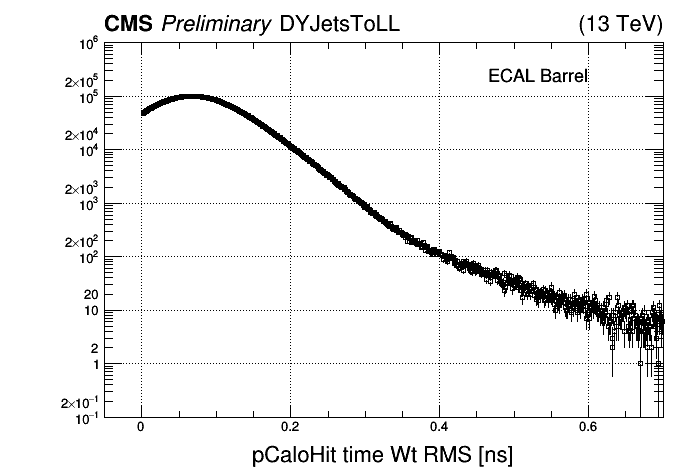
\includegraphics{fig/sec_gen/tr_pcaloWtRMS_hist_07012021124909.png}}
\caption{The event by event Wt. RMS for the pCaloHit times geometrically matched to individual crystals for all crystal in EB. In crystals with a multiplicity greater than one, the Wt. RMS is shown to peak at $\sim$60-80 ps.}
\label{pc_rms}
\end{center}
\end{figure}

The correlations between the sum of the pCaloHit energies, the multiplicity, and the Wt.RMS, as shown in Figure~\ref{pc_sevm}, within the pCaloHits geometrically matched to a crystal were studied. As can be seen in the plot on the top left in Figure~\ref{pc_sevm}, the crystals with larger sums of pCaloHit energies correspond to those with higher multiplicities, as would be expected in terms of shower development. In the top right plot we can see that there is no strong apparent correlation between the sum of the pCaloHit energies in a crystal and the Wt. RMS of the pCaloHit times in that crystal. In the plot on the bottom it can be seen that the Wt. RMS of the pCaloHit times have characteristic range of approximately 80-100 ps that is persistent with increasing multiplicity.

\begin{figure}[htbp]
\begin{center}
%\resizebox{0.48\textwidth}{!}{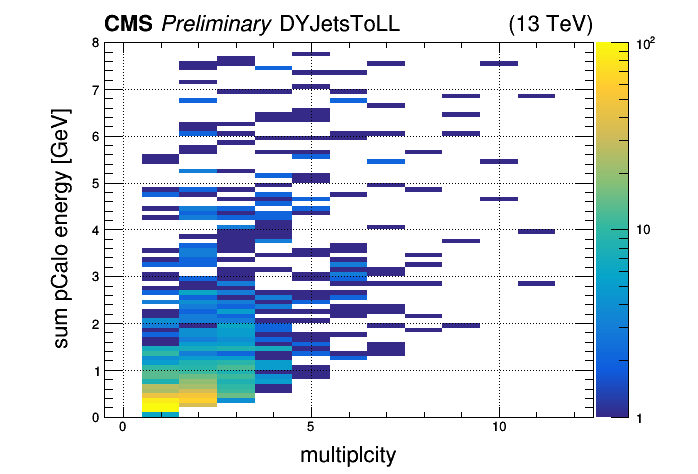
\includegraphics{fig/sec_gen/tr_2d_multi_v_sume_12112020155403.png}}
\resizebox{0.475\textwidth}{!}{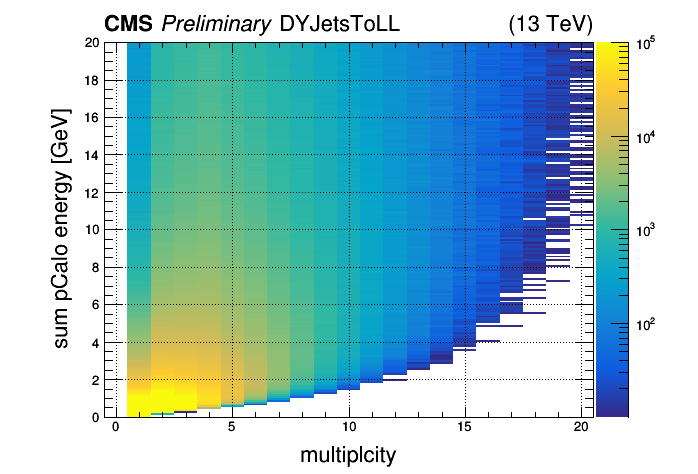
\includegraphics{fig/sec_gen/tr_2d_spcevmulti_07012021143040.png}}
\resizebox{0.475\textwidth}{!}{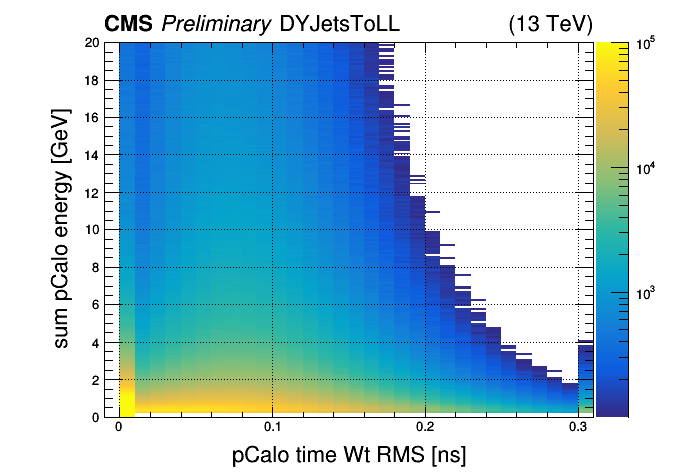
\includegraphics{fig/sec_gen/tr_2d_pcrmsvspce_07012021142215.png}}
\resizebox{0.475\textwidth}{!}{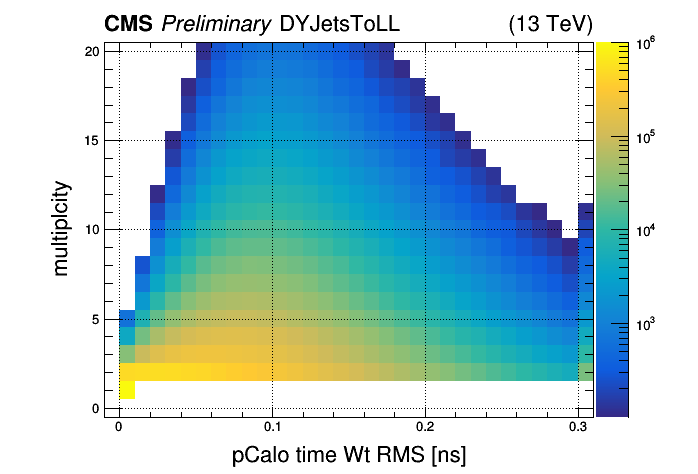
\includegraphics{fig/sec_gen/tr_2d_pcrmsvmulti_07012021142611.png}}
\caption{The correlations between the sum of the pCaloHit energy and the multiplicity (top left), the  Wt. RMS of the pCaloHit times and the sum of the pCaloHit energy (top right), and the Wt. RMS of the pCaloHit times and the pCaloHit multiplicity (bottom) for pCaloHits geometrically matched to a crystal. }
\label{pc_sevm}
\end{center}
\end{figure}

%\begin{figure}[htbp]
%\begin{center}
%\resizebox{0.48\textwidth}{!}{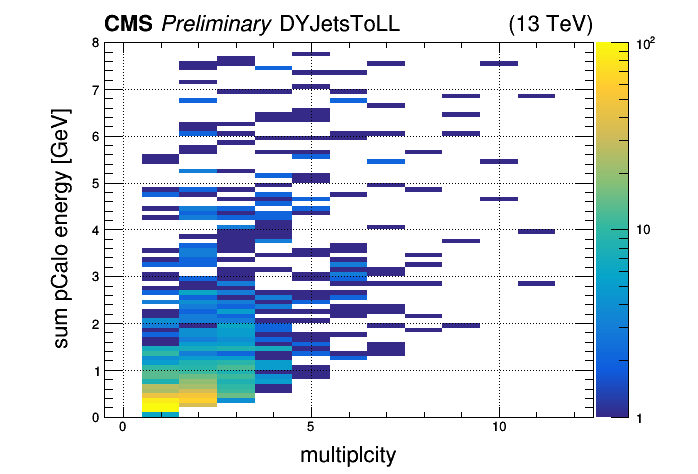
\includegraphics{fig/sec_gen/tr_2d_multi_v_sume_12112020155403.png}}
%\resizebox{0.48\textwidth}{!}{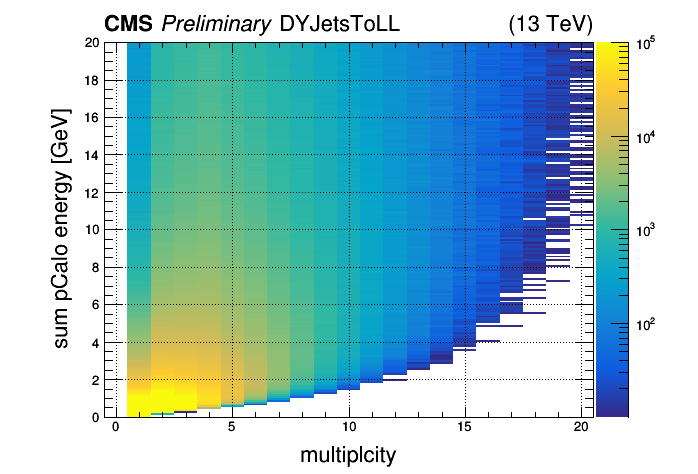
\includegraphics{fig/sec_gen/tr_2d_spcevmulti_07012021143040.png}}
%\caption{Sum pCaloHit energy correlated to pCaloHit multiplicity. }
%\label{pc_sevm}
%\end{center}
%\end{figure}

%\begin{figure}[htbp]
%\begin{center}
%\resizebox{0.48\textwidth}{!}{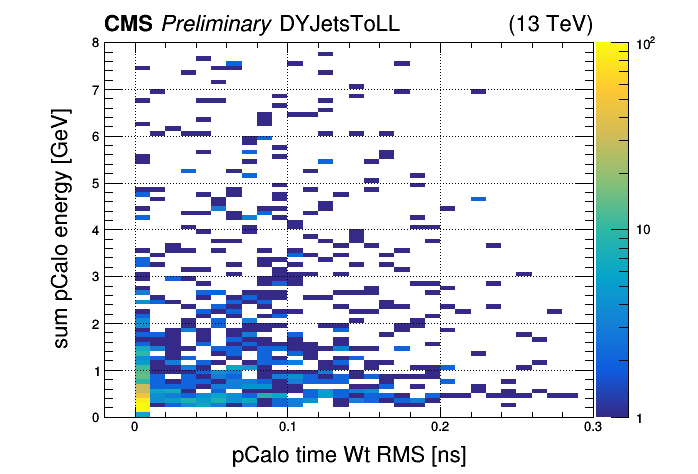
\includegraphics{fig/sec_gen/tr_2d_wtrms_v_sume_12112020155004.png}}
%\resizebox{0.48\textwidth}{!}{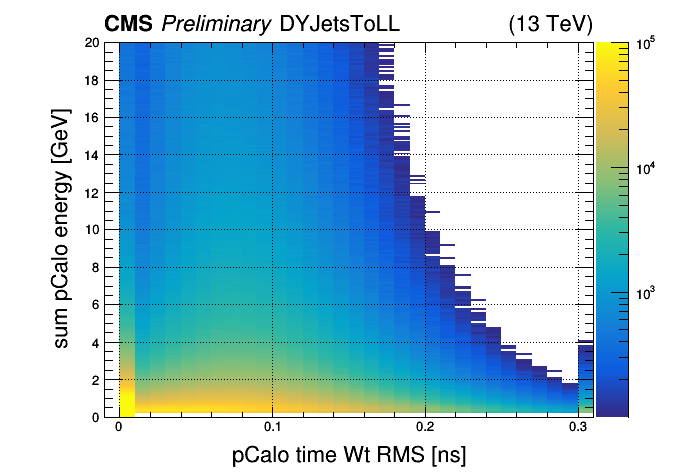
\includegraphics{fig/sec_gen/tr_2d_pcrmsvspce_07012021142215.png}}
%\caption{Sum pCaloHit energy correlated to pCaloHit time weighted RMS. }
%\label{pc_sevrms}
%\end{center}
%\end{figure}

%\begin{figure}[htbp]
%\begin{center}
%\resizebox{0.48\textwidth}{!}{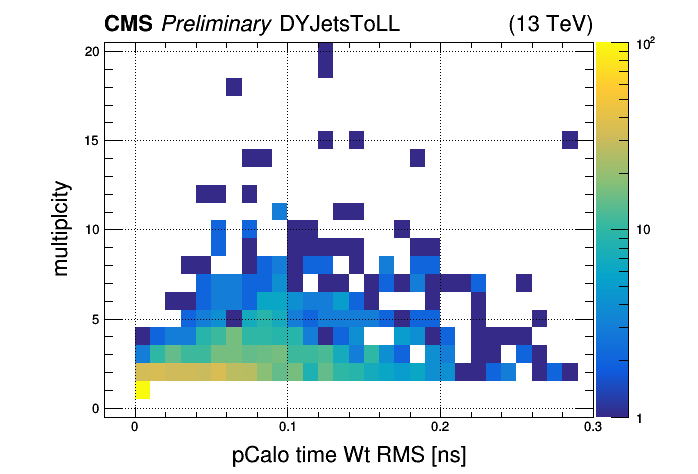
\includegraphics{fig/sec_gen/tr_2d_wtrms_v_multi_12112020154432.png}}
%\resizebox{0.48\textwidth}{!}{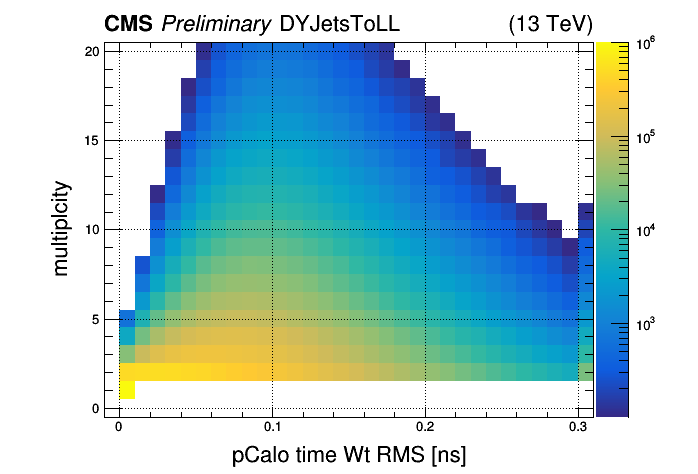
\includegraphics{fig/sec_gen/tr_2d_pcrmsvmulti_07012021142611.png}}
%\caption{pCaloHit multiplicity correlated to pCaloHit time weighted RMS. }
%\label{pc_mvrms}
%\end{center}
%\end{figure}

The gen time for a rechit is calculated as the energy weighted average of the pCaloHit times that have an pCaloHit energy of at least 100 MeV for all pCaloHits geometrically matched to the crystal the rechit was in, as shown in Equation~\ref{eq_gentime}.

\begin{equation} 
\emph{Gen Time} = \frac{\sum( pCaloHit time * pCaloHit energy )}{\sum pCaloHit energy }
\label{eq_gentime}
\end{equation}

The distribution of the gen times in the same four crystals that were previously referenced are shown in Figure~\ref{pc_4c_wat}. Since the actual values recorded for the pCaloHit times are the time since the bunch crossing at CMS origin at which an interacting particle deposited the energy if the pCaloHit in a particular crystal, the pCAloHit times in the EB are expected to vary from $\sim$4-12 ns. The distribution of the weighted average pCaloHit times seen in Figure~\ref{pc_4c_wat} are consistent with the expected mean time given the geometrical location of the selected crystals. In Figure~\ref{pc_wat} the gen times for all EB crystal where the corresponding rechit energy is between 10 GeV and 120 GeV is shown. Consistent with the distributions seen in Figure~\ref{pc_4c_wat} for a single crystal, the time distribution spreads between five and ten nanoseconds as expected, given the time of flight from the CMS origin to the physical location of the crystals.

\hfill
\begin{figure}[htbp]
\begin{center}
\resizebox{0.45\textwidth}{!}{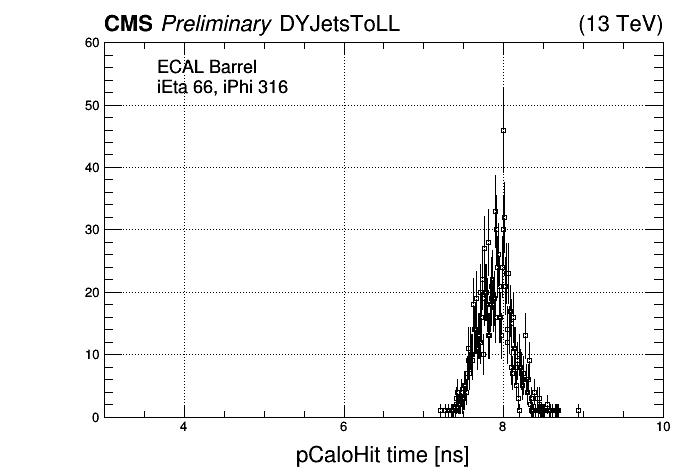
\includegraphics{fig/sec_gen/tr_pcaloMtime0_hist_23112020160113.png}}
\resizebox{0.45\textwidth}{!}{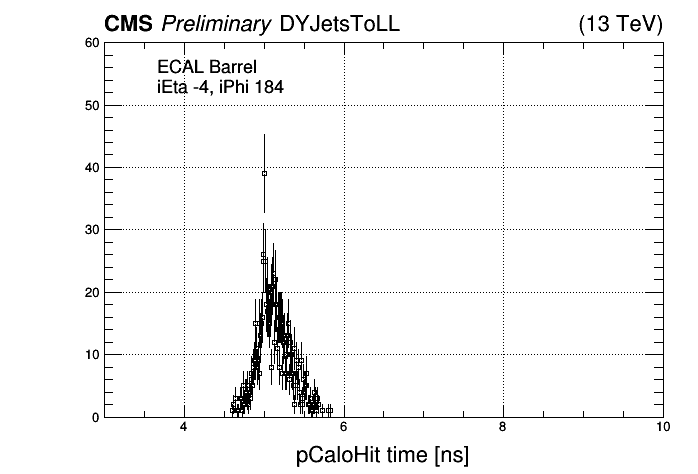
\includegraphics{fig/sec_gen/tr_pcaloMtime1_hist_23112020160311.png}}
\resizebox{0.45\textwidth}{!}{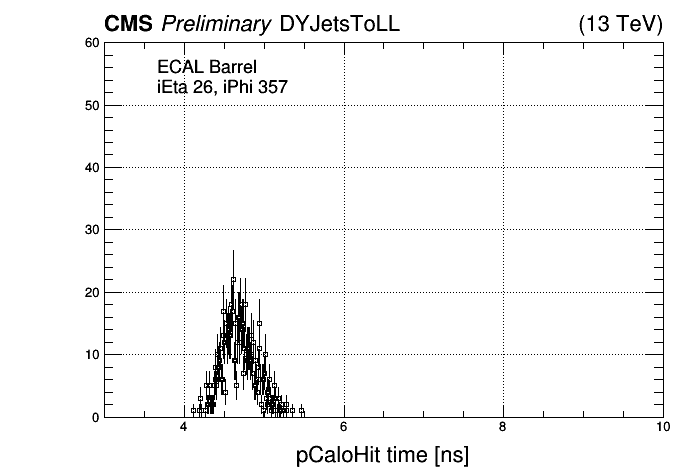
\includegraphics{fig/sec_gen/tr_pcaloMtime2_hist_23112020160510.png}}
\resizebox{0.45\textwidth}{!}{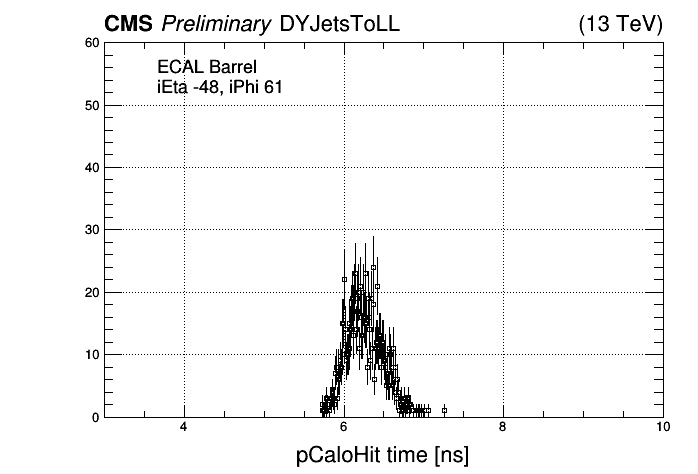
\includegraphics{fig/sec_gen/tr_pcaloMtime3_hist_23112020160828.png}}
\caption{Weighted average pCaloHit time, or gen time, in the four separate crystal of the pCalo hits geometrically matched to those crystals. These crystals are located, in order left to right, top to bottom, at (ieta, iphi) of : (66,316), (26,357), (-4,184), and (-48,61) in the EB.} 
\label{pc_4c_wat}
\end{center}
\end{figure} 

%\begin{figure}[htbp]
%\begin{center}
%\resizebox{0.42\textwidth}{!}{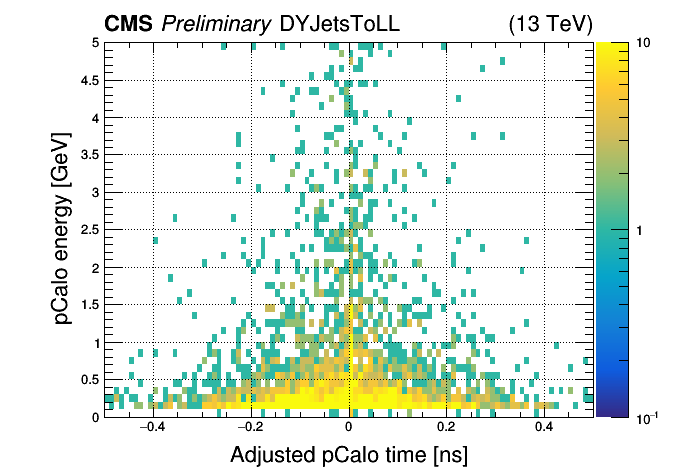
\includegraphics{fig/sec_gen/tr_2d_pctve_24112020141604.png}}
%\resizebox{0.42\textwidth}{!}{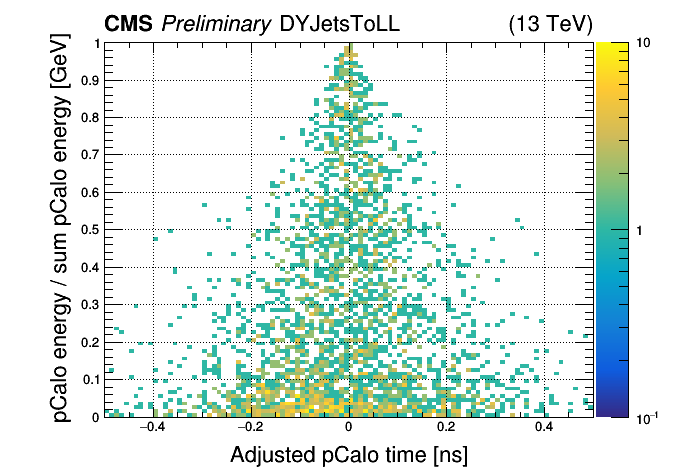
\includegraphics{fig/sec_gen/tr_2d_pctvne_24112020141913.png}}
%\resizebox{0.42\textwidth}{!}{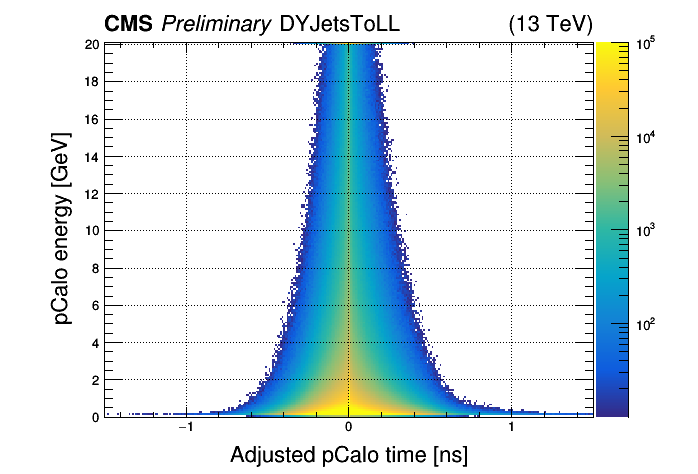
\includegraphics{fig/sec_gen/tr_2d_apctvpce_07012021145909.png}}
%\resizebox{0.42\textwidth}{!}{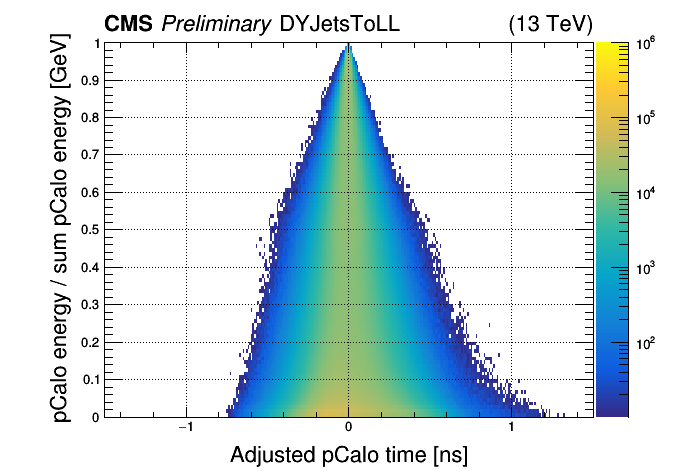
\includegraphics{fig/sec_gen/tr_2d_apctvnpce_07012021150111.png}}
%\caption{Adjusted pCaloHit time [ns] with respect to pCalo energy [GeV]. The pCalo time is adjusted by subtracting the weighted average time of the pCalo hits from the time of the individual pCalo hits. In the right hand plot the pCalo energy is normalized by the sum of the pCalo energies.}
%\label{pc_adjtve}
%\end{center}
%\end{figure} 

%\begin{figure}[htbp]
%\begin{center}
%\resizebox{0.42\textwidth}{!}{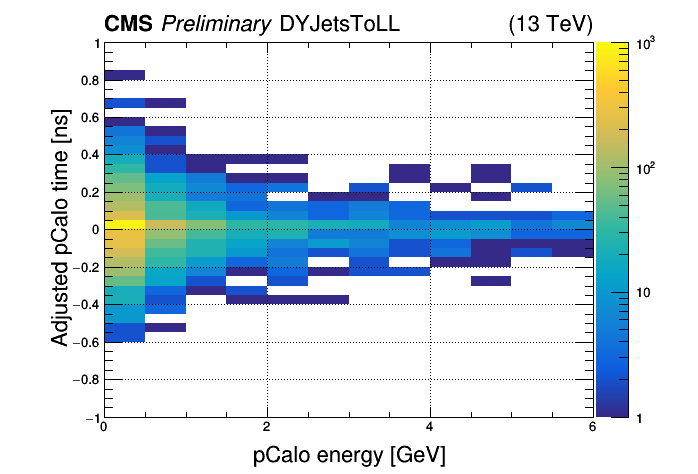
\includegraphics{fig/sec_gen/tr_pcalo_calitve_hist_17112020185058.png}}
%\resizebox{0.42\textwidth}{!}{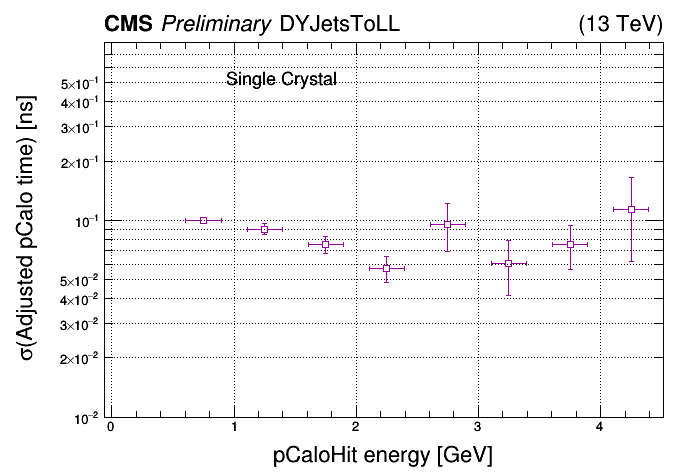
\includegraphics{fig/sec_gen/tr_mc_sp_plot_17112020185336.png}}
%\resizebox{0.42\textwidth}{!}{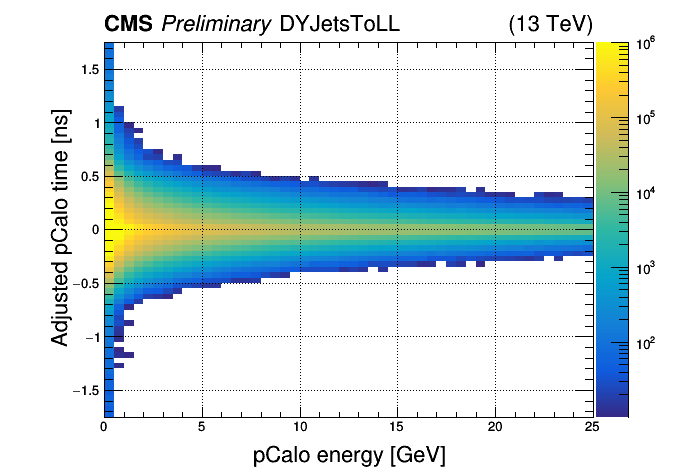
\includegraphics{fig/sec_gen/tr_2d_mcDataHist_13012021134816.png}}
%\resizebox{0.42\textwidth}{!}{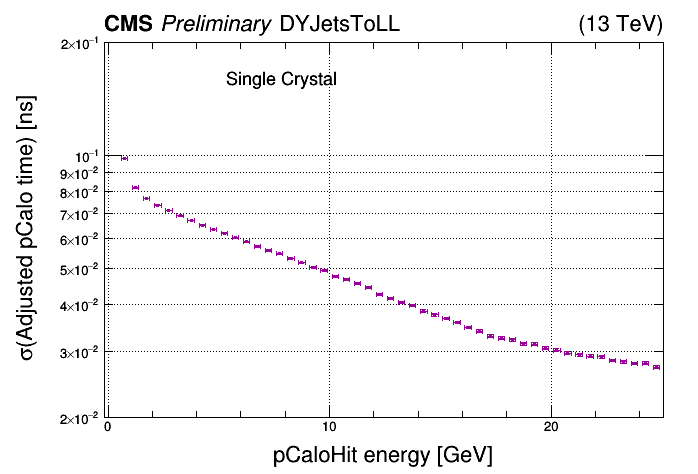
\includegraphics{fig/sec_gen/tr_mc_sp_plot_19012021181820.png}}
%\caption{Single crystal time distribution widths of adjusted pCalo times [ns] with respect to pCalo energy [GeV].}
%\label{pc_pctve_scres}
%\end{center}
%\end{figure} 

The times reconstructed by the timing algorithms, once calibrated, are shifted so that the average time of all hits in a particular crystal is zero. This effectively shifts the mean time of a rechit in each crystal to be zero with respect to the time that the bunch crossing theoretically occurs at the CMS origin. In order to compare the pCalo gen times to the rechit times it is necessary to shift the gen times so that the gen time and the rechit time are both in the same temporal frame of reference. The gen times include the difference in time between the theoretical BX time at the origin and the time that an interaction occurred in the crystal, as well as the the flight time for a particle from the interaction vertex to the physical location of the crystals. To account for the difference between the actual interaction vertex for an event and the rechit time in a global resolution study, the rechit times are TOF corrected from the CMS origin to the physical location of the crystal in which the rechit occurs and are then TOF shifted from the crystal location to the location of the PV. This effectively regresses the time of the rechit back to the time when the particle that produced the rechit was created. To bring the gen times into the same temporal frame of reference they are TOF shifted from the physical crystal location to the position of the PV, therefore also shifting the gen time from the time of the particle interaction with the crystal to the time that the particle which interacted with the crystal was theoretically produced in the PV. In the case of a local resolution study, the TOF correction are also made to the rechit times but have a negligible impact on the local resolution.

\begin{figure}[htbp]
\begin{center}
\resizebox{0.7\textwidth}{!}{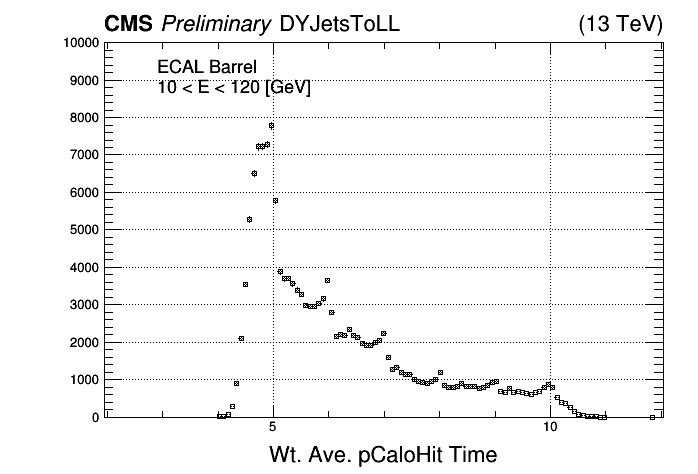
\includegraphics{fig/sec_gen/tr_pcalo_raw_wt_ave_time_hist_15122020161151.png}}
\caption{Gen time for rechits with energies between 10 GeV and 120 GeV in the EB. The gen time distribution is spread between $\sim$4-12 ns, as is to be expected given the time of flight from the CMS origin to the physical location of the crystals.}
\label{pc_wat}
\end{center}
\end{figure}

Using the gen time obtained from the TOF adjusted average weighted pCalo time as a truth time has several limitations. As mentioned previously, the depth of the energy deposition recorded by the pCalo hits does not preserve the information of the depth of deposition in the crystal. The pCalo hits do not reflect the variations arising from the location of the hit on the crystal face or the light collection efficiency of the crystal, and the TOF adjustments are sensitive to the resolution of the primary vertex. These limiting factors mean that it is not possible to archive a perfect resolution with this method of producing a truth time. As can be seen in Figure~\ref{pc_scres}, though, approximately the same resolution is achieved across all energies, for both the Same RO unit and the $Z\rightarrow e^{+}e^{-}$ cases, of $\sim$80-90 ps.

\begin{figure}[htbp]
\begin{center}
\resizebox{0.7\textwidth}{!}{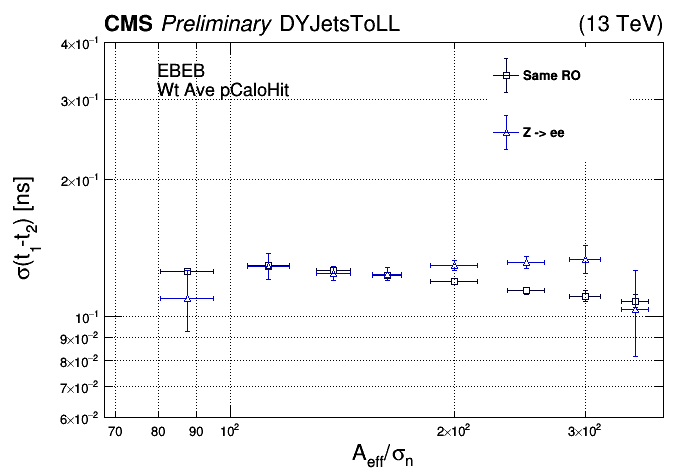
\includegraphics{fig/sec_gen/tr_mc_lgres_plot_15112021155242.png}}
\caption{Same RO and $Z\rightarrow e^{+}e^{-}$ resolutions in DYjetsToLL MC for pCAlo gen time. Roughly the same resolution of $\sim$80-90 ps is achieved across all energies for both the Same RO unit and the $Z\rightarrow e^{+}e^{-}$ cases.} 
\label{pc_scres}
\end{center}
\end{figure} 

Since the data used as input for the timing reconstruction methods is derived from the pCaloHit collection, the resolution obtained using the pCaloHit gen time reference is the best resolution achievable by the timing reconstruction with a particular MC data stream. 


%********* intros PV resolution and crystal face hit location approximation effects to gen time resolutions ... 
% ... only explain our method of obtaining a gen time then -> see below .....
%.... make statements about limitations in current gen times from pcalo from most recent gen time studies talk in ecal moca meeting Apr 28 2021 ....
%... end section with pcalo vs cc \& ratio single crystal resolutions in MC ......




%\begin{figure}[htbp]
%\begin{center}
%\resizebox{0.22\textwidth}{!}{\includegraphics{fig/sec_gen/tr_pcalo}}
%\resizebox{0.22\textwidth}{!}{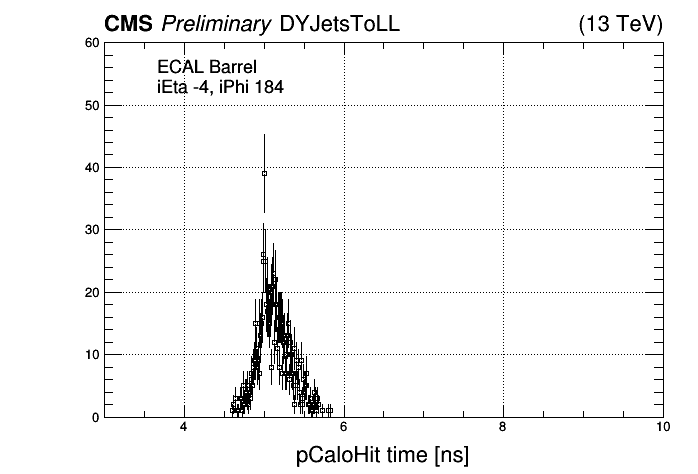
\includegraphics{fig/sec_gen/tr_pcaloMtime1_hist_23112020160311.png}}
%\resizebox{0.22\textwidth}{!}{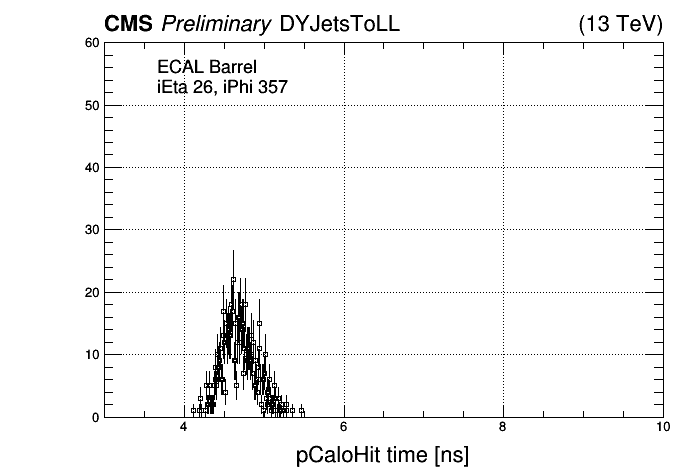
\includegraphics{fig/sec_gen/tr_pcaloMtime2_hist_23112020160510.png}}
%\resizebox{0.22\textwidth}{!}{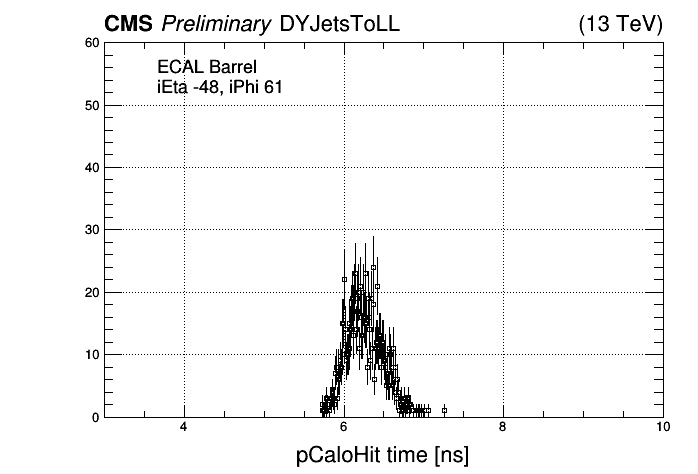
\includegraphics{fig/sec_gen/tr_pcaloMtime3_hist_23112020160828.png}}
%\caption{pCaloHit energy in the four separate crystals studied. } 
%\label{pc_4c_pce}
%\end{center}
%\end{figure} 


\FloatBarrier

\section{ECAL Timing Performance \label{sec:res}}
\subsection{Resolution \label{sec:resmeth1}}
Resolution studies are used to quantify the precision of a timing reconstruction method.
The time resolution is determined from the difference between the reconstructed times of two hits (rechits) that are expected to be produced simultaneously.
Two complementary methods are employed to select such pairs of rechits, as illustrated in Fig.~\ref{trm_local_global_xstal}.

The first method selects a pair of adjacent crystals with similar energies within a single electromagnetic (EG) candidate cluster and is used to measure a \emph{local resolution}.
This approach probes the intrinsic single-crystal timing performance and provides sensitivity to delays arising from the readout electronics.
The second method selects a pair of rechits associated with electrons from a reconstructed $Z \rightarrow e^{+}e^{-}$ decay.
This \emph{global resolution} reflects the timing performance relevant for physics analyses, where hits originate from spatially separated regions of the detector.

\begin{figure}[htbp]
\begin{center}
\resizebox{0.7\textwidth}{!}{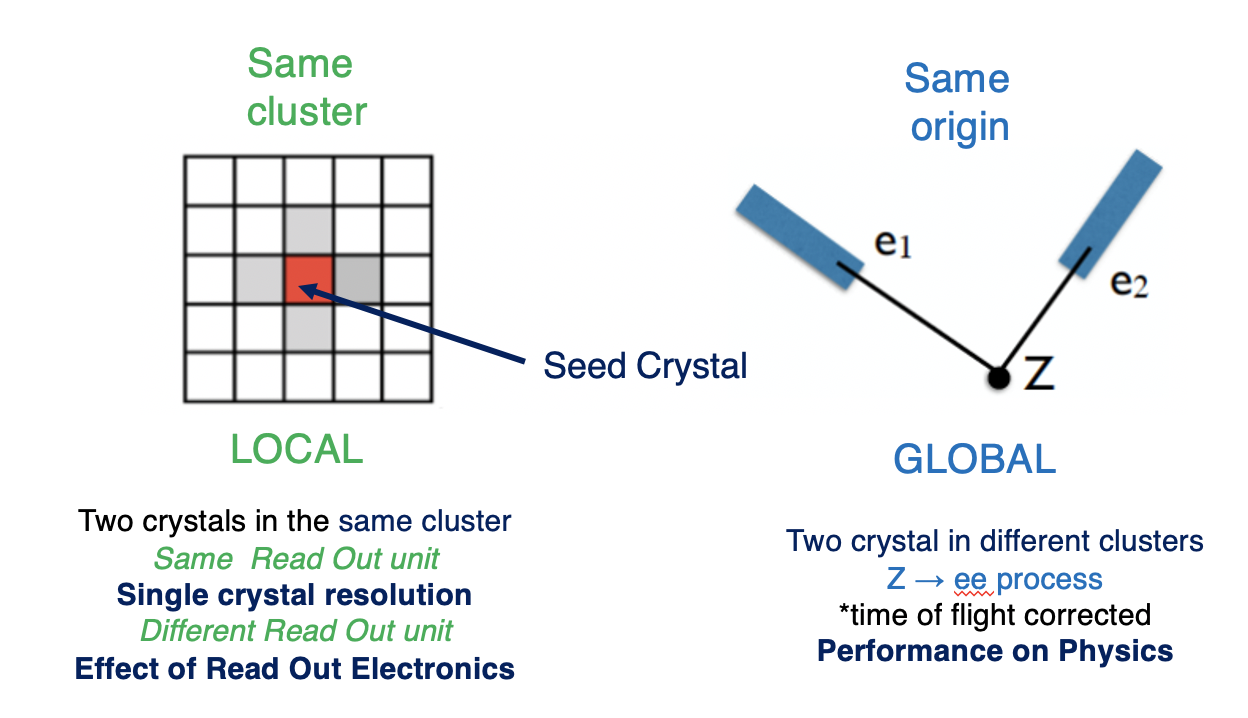
\includegraphics{fig/sec_method/Local_global_crystals.png}}
\caption{Methods used to select crystal pairs for time resolution measurements.
For the local resolution (right), two adjacent crystals within the same cluster are selected.
For the global resolution (left), seed crystals from two clusters associated with electrons from a $Z \rightarrow e^{+}e^{-}$ decay are used.}
\label{trm_local_global_xstal}
\end{center}
\end{figure}

For the local resolution, a pair of rechits is selected from the crystal cluster forming an EG candidate.
One crystal is required to be the seed crystal of the cluster, while the second must be an adjacent crystal in either the $\eta$ or $\phi$ direction.
The energy of the adjacent crystal is required to be within 20\,\% of the seed-crystal energy.
The EG candidate is further required to satisfy shower-shape criteria, with the semi-minor axis of the second moment of the cluster geometry satisfying $\texttt{smin} < 0.3$ and the semi-major axis satisfying $\texttt{smaj} < 0.5$.
If multiple EG candidates in an event satisfy these criteria, the candidate with the largest momentum is selected.

Local resolutions are further categorized based on whether the two crystals share the same readout electronics.
If both crystals are located within the same trigger tower, the measurement is referred to as a \emph{same readout unit} (\textbf{SRU}) resolution.
If the crystals are located in adjacent trigger towers, the measurement is referred to as a \emph{different readout unit} (\textbf{DRU}) resolution.
These local resolution categories probe both intrinsic detector timing performance and effects arising from readout electronics and pileup.

For the global resolution, seed crystals from two EG candidates matched to electrons from a $Z \rightarrow e^{+}e^{-}$ decay are selected.
Each EG candidate is required to be matched to an electron with $\Delta R < 0.1$, and the electron track $z$ position must be within 0.05\,cm of the primary-vertex $z$ position.
Pairs of EG candidates with an invariant mass between 60 and 150\,GeV are considered, and if multiple qualifying pairs are present, the pair with invariant mass closest to the nominal $Z$ boson mass is selected.

For the global resolution, a correction is applied to account for the difference in time-of-flight (TOF) of the two electrons from the primary vertex to their respective seed-crystal positions.
The resulting measurement is referred to as the \emph{$Z \rightarrow e^{+}e^{-}$} (\textbf{ZEE}) resolution.
The selection criteria used for the SRU, DRU, and ZEE resolution measurements are summarized in Table~\ref{res_params}.

As illustrated in Fig.~\ref{trm_timeproccess}, the time difference between the two selected rechits,
$\Delta(\text{Seed Time}) = t_{1} - t_{2}$,
is evaluated as a function of an effective amplitude, $A_{\mathrm{eff}} / \sigma_{N}$, which is proportional to the energy of the corresponding EG candidates.
The effective amplitude is defined as
\begin{equation}
A_{\mathrm{eff}}/\sigma_{N} =
\frac{(A_{1}/\sigma_{N_{1}})(A_{2}/\sigma_{N_{2}})}
{\sqrt{(A_{1}/\sigma_{N_{1}})^{2} + (A_{2}/\sigma_{N_{2}})^{2}}} \, ,
\label{eq_a}
\end{equation}
where $A_{i}$ is the pulse amplitude measured in crystal $i$ and $\sigma_{N_{i}}$ is the corresponding pedestal noise.

The distribution of $\Delta(\text{Seed Time})$ is formed in bins of $A_{\mathrm{eff}}/\sigma_{N}$ and fitted with a Gaussian function.
The standard deviation $\sigma(t_{1}-t_{2})$ extracted from each fit is then plotted as a function of the central value of the corresponding $A_{\mathrm{eff}}/\sigma_{N}$ bin.

\begin{figure}[htbp]
\begin{center}
\resizebox{0.95\textwidth}{!}{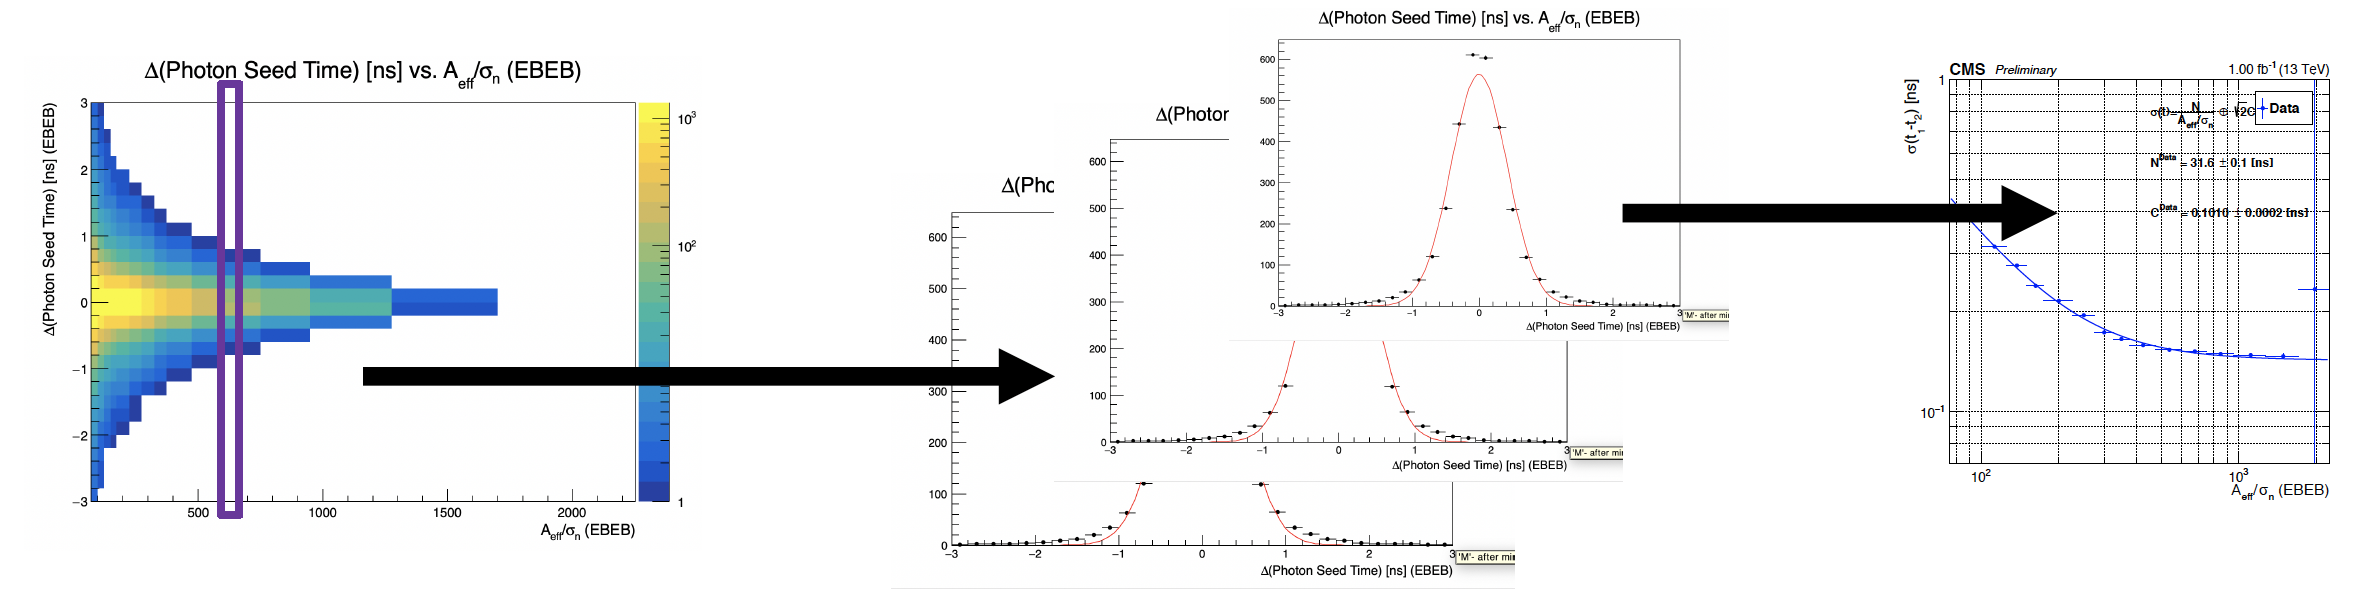
\includegraphics{fig/sec_method/timeres_process.png}}
\caption{Procedure used to extract the time resolution.
The distribution of $\Delta(\text{Seed Time})$ is formed in bins of $A_{\mathrm{eff}}/\sigma_{N}$ and fitted with a Gaussian.
The extracted standard deviation $\sigma(t_{1}-t_{2})$ is plotted as a function of $A_{\mathrm{eff}}/\sigma_{N}$ and fitted using the resolution parameterization described in the text.}
\label{trm_timeproccess}
\end{center}
\end{figure}

The dependence of $\sigma(t_{1}-t_{2})$ on $A_{\mathrm{eff}}/\sigma_{N}$ characterizes the time resolution and is traditionally described by
\begin{equation}
\sigma^{2}_{i} =
\left(\frac{N}{A_{\mathrm{eff}}/\sigma_{N}}\right)^{2} + 2C^{2} \, ,
\label{eq_b}
\end{equation}
where $N$ parameterizes the contribution from electronic noise and $C$ is a constant term.
The constant term includes contributions from variations in shower development within the crystal, crystal-to-crystal differences in pulse shapes, readout-unit-dependent delays, and pileup effects.
For each resolution category (SRU, DRU, and ZEE), the constant term $C$ represents the asymptotic timing resolution at high signal amplitude.

To better describe the resolution behavior at lower effective amplitudes, the parameterization can be extended to include a stochastic term,
\begin{equation}
\sigma^{2}_{i} =
\left(\frac{N}{A_{\mathrm{eff}}/\sigma_{N}}\right)^{2}
+ \frac{S^{2}}{A_{\mathrm{eff}}/\sigma_{N}}
+ 2C^{2} \, ,
\label{eq_c}
\end{equation}
where $S$ captures additional fluctuations that scale inversely with signal amplitude.
While this term is not traditionally included, its addition improves the quality of the fit when extending the analysis to lower values of $A_{\mathrm{eff}}/\sigma_{N}$.
This extended parameterization is used for resolution measurements performed with the CC timing reconstruction.

\hfill
\begin{table}[h!]
\begin{center}
 \begin{tabular}{ |c| }
 \hline
 Resolution Selection Cuts \\
 \hline
 \hline
 Local Resolution\\
 \hline
  %isOOT false \\
  %At least one photon candidate \\
  Photon smin $>$ 0.3 \\
  Photon smaj $>$ 0.5 \\
  %choose a seed crystal and an adjacent crystal to the seed crystal\\ 
  Photon seed crystal has an adjacent crystal where : \\ 
  seed crystal energy $<$ 120\% adjacent crystal energy \\
  Qualifying seed crystal with largest energy \\
 \hline
 Global Resolution\\
 \hline
  Photon has PixSeed \\
  Photon gedID $<$ 3 \\
  %isOOT false \\
  Photon matches to an electron with dR $<$ 0.1  \\
  Matching electron has trackZ within 1.0 cm of primary vertex Z \\
  At least 2 qualifying photons \\
  Pair of photons with combined mass $<$ 150 GeV \& $>$ 60 GeV \\
  Qualifying pair of photons with combined mass closets to Z mass \\
\hline
\end{tabular}
\end{center}
\caption{Selection cuts for local and global resolutions.}
\label{res_params}
\end{table}
%redone
\FloatBarrier
\subsection{Calibration \label{sec:resmeth3}}
\begin{figure}[htbp]
\begin{center}
\resizebox{0.7\textwidth}{!}{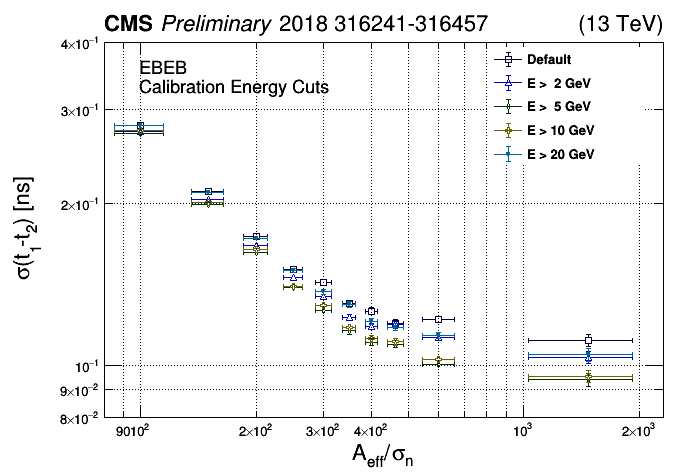
\includegraphics{fig/sec_method/tr_kucc_18s_ecut_v25_01122021174016.png}}
\caption{Same readout unit (SRU) resolution obtained with the default CMSSW timing reconstruction after applying an external calibration.
The calibration constants are derived by averaging rechit times on a channel-by-channel basis using rechits with energy greater than a specified threshold.}
\label{e5cali}
\end{center}
\end{figure}

To enable a consistent comparison between different ECAL timing reconstruction algorithms, rechit times must be calibrated using a common procedure.
During Run~II development, it was not possible to apply the default CMSSW timing calibration framework directly to rechits reconstructed with the CC algorithm.
An external calibration procedure based on the average rechit time per channel was therefore implemented.

In this approach, calibration constants are derived by computing the mean rechit time for each crystal over a selected set of events.
To suppress contributions from electronic noise and poorly reconstructed pulses, rechits used in the calibration are required to exceed a minimum energy threshold.
The dependence of the resulting timing resolution on this threshold was studied using the default CMSSW timing reconstruction in selected runs from the 2018D data-taking period.

As shown in Fig.~\ref{e5cali}, increasing the minimum rechit energy threshold above 5\,GeV yields negligible improvement in the calibrated time resolution.
Based on these studies, a threshold of 5\,GeV is chosen for the external calibration procedure.
This calibration is applied to all rechit times reconstructed with the CC algorithm throughout this analysis and is used consistently for Run~II studies prior to the introduction of a CC-specific calibration within CMSSW during Run~III.

For direct comparisons between the CC and ratio-based timing reconstructions, an analogous external calibration derived from rechit times reconstructed with the ratio method is also applied.
This ensures that both timing algorithms are calibrated using equivalent procedures and that observed differences in performance reflect intrinsic reconstruction behavior rather than calibration effects.
%redone
\FloatBarrier
\subsection{Performance of Cross Correlation Algorithm in Data \label{sec:resdata}}
Out-of-time pileup (OOT-PU) arises when energy deposits originating from interactions in preceding bunch crossings contribute to the signal recorded in the current bunch crossing.
Since the scintillation pulse produced in ECAL crystals extends beyond the 25~ns bunch spacing, signals from multiple bunch crossings can overlap and distort the reconstructed pulse shape.
This effect degrades the timing reconstruction and introduces dependencies on both the bunch-crossing (BX) position within a filled train and the signal amplitude.

The impact of OOT-PU on the time reconstruction can be studied by examining the mean rechit time as a function of the BX position within a train of filled buckets.
Figure~\ref{cclhcplots1} shows the mean rechit time by BX for rechits reconstructed with the ratio and CC algorithms, for minimum rechit energies of 2~GeV and 20~GeV.
For this comparison, rechit times are calibrated by subtracting the mean time averaged over all BXs for rechits with energy greater than 5~GeV in the corresponding collection.

\begin{figure}[h!tbp]
\begin{center}
\resizebox{0.7\textwidth}{!}{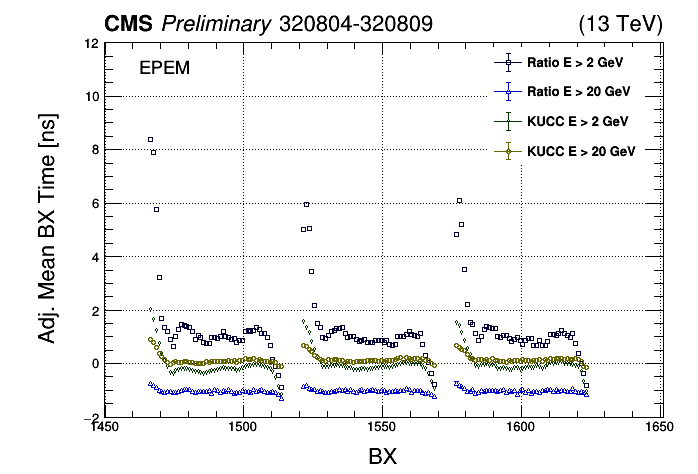
\includegraphics{fig/sec_results/tr_lhc_18A_v25_talk_30112021151421.png}}
\caption{Mean rechit time as a function of bunch-crossing position within a typical train of filled buckets, shown for the ratio and CC timing reconstructions.
Results are shown for minimum rechit energies of 2~GeV and 20~GeV.
The CC algorithm exhibits a reduced dependence on BX position and a significantly smaller energy dependence than the ratio method, demonstrating improved mitigation of OOT pileup.}
\label{cclhcplots1}
\end{center}
\end{figure}

In the leading and trailing regions of the bunch trains, the CC algorithm substantially reduces the dependence of the reconstructed time on BX position compared to the ratio algorithm.
In the central region of the trains, the separation between the 2~GeV and 20~GeV samples is significantly smaller for the CC reconstruction, indicating a markedly reduced energy dependence.
Together, these features demonstrate the improved robustness of the CC algorithm against OOT-PU effects across the full bunch train.

During the development of the CC reconstruction in Run~II, a two-tier processing strategy was employed in which rechit collections produced with both the CC and ratio algorithms were stored simultaneously.
This approach enabled a direct, event-by-event comparison of the two timing methods using identical detector conditions and reconstruction inputs.
Performance studies were carried out in both simulation and recorded data using this strategy.

The intrinsic performance of the CC algorithm was first studied in simulation by comparing its resolution to that obtained with the ratio algorithm and to the generator-level timing information derived from \texttt{pCaloHits}.
Since the reconstructed pulses used by the timing algorithms are simulated from \texttt{pCaloHits}, the resolution obtained using the generator-level time provides a reasonable estimate of the optimal achievable performance.
Figure~\ref{pc_rt_cc_comp} shows the single-crystal same readout unit (SRU) resolution as a function of effective amplitude for the ratio algorithm, the CC algorithm, and the generator-level reference.
The CC algorithm exhibits a significantly narrower resolution than the ratio method across the full amplitude range and approaches the generator-level resolution at high effective amplitudes.

\begin{figure}[h!tbp]
\begin{center}
\resizebox{0.7\textwidth}{!}{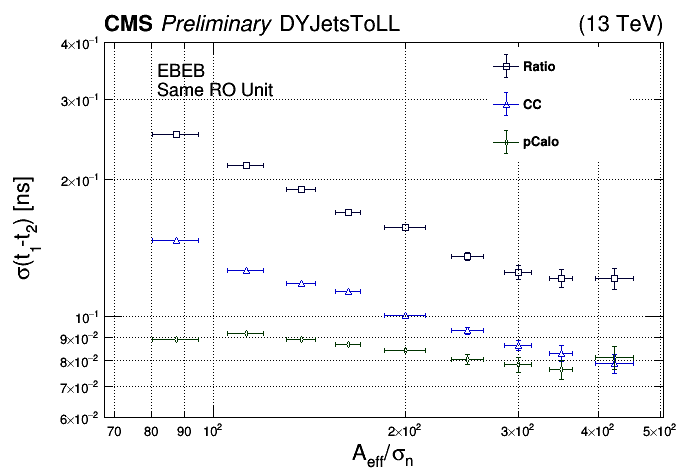
\includegraphics{fig/sec_gen/tr_mc_pc2_loc_plot_30112021153817.png}}
\caption{Single-crystal same readout unit (SRU) resolution in simulation for the ratio algorithm, the CC algorithm, and generator-level (\texttt{pCaloHit}) timing.
The CC algorithm achieves a significantly improved resolution relative to the ratio method and approaches the generator-level resolution at high effective amplitudes.}
\label{pc_rt_cc_comp}
\end{center}
\end{figure}

Figure~\ref{ccresr2} shows the same readout unit (SRU) and $Z \rightarrow e^{+}e^{-}$ object-level (ZEE) timing resolutions measured in Run~II data using the two-tier processing approach and external calibrations.
The CC algorithm improves the SRU resolution by approximately 30~ps and the ZEE resolution by approximately 35~ps relative to the ratio algorithm.

\begin{figure}[h!tbp]
\begin{center}
\resizebox{0.7\textwidth}{!}{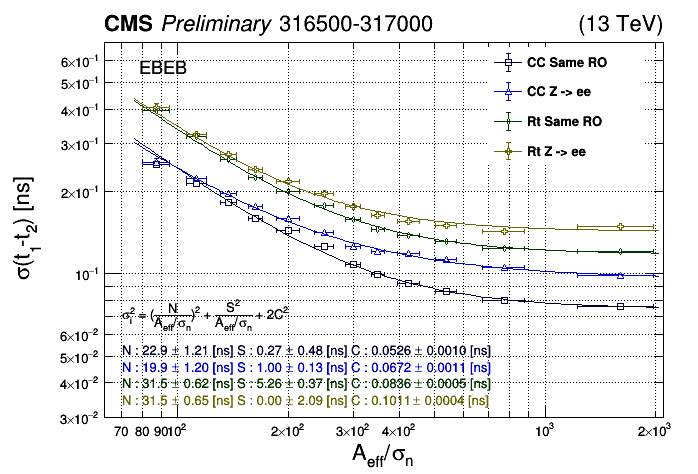
\includegraphics{fig/sec_results/tr_kucc_18As_v25_talk_30112021160215.png}}
\caption{Comparison of same readout unit (SRU) and $Z \rightarrow e^{+}e^{-}$ object-level (ZEE) timing resolutions for the ratio and CC algorithms in Run~II data, using two-tier processing and external calibrations.
The CC algorithm improves the SRU resolution by approximately 30~ps and the ZEE resolution by approximately 35~ps.}
\label{ccresr2}
\end{center}
\end{figure}

In Run~III, the CC timing algorithm was fully integrated into CMSSW and a dedicated online calibration was introduced.
Figure~\ref{ccresr3} compares the timing resolutions obtained from two independent prompt reconstructions of the same Run~III dataset, one using the ratio method and the other using the CC method as the default time reconstruction.
An improvement of approximately 80~ps in the SRU resolution is observed for the CC reconstruction.

\begin{figure}[h!tbp]
\begin{center}
\resizebox{0.7\textwidth}{!}{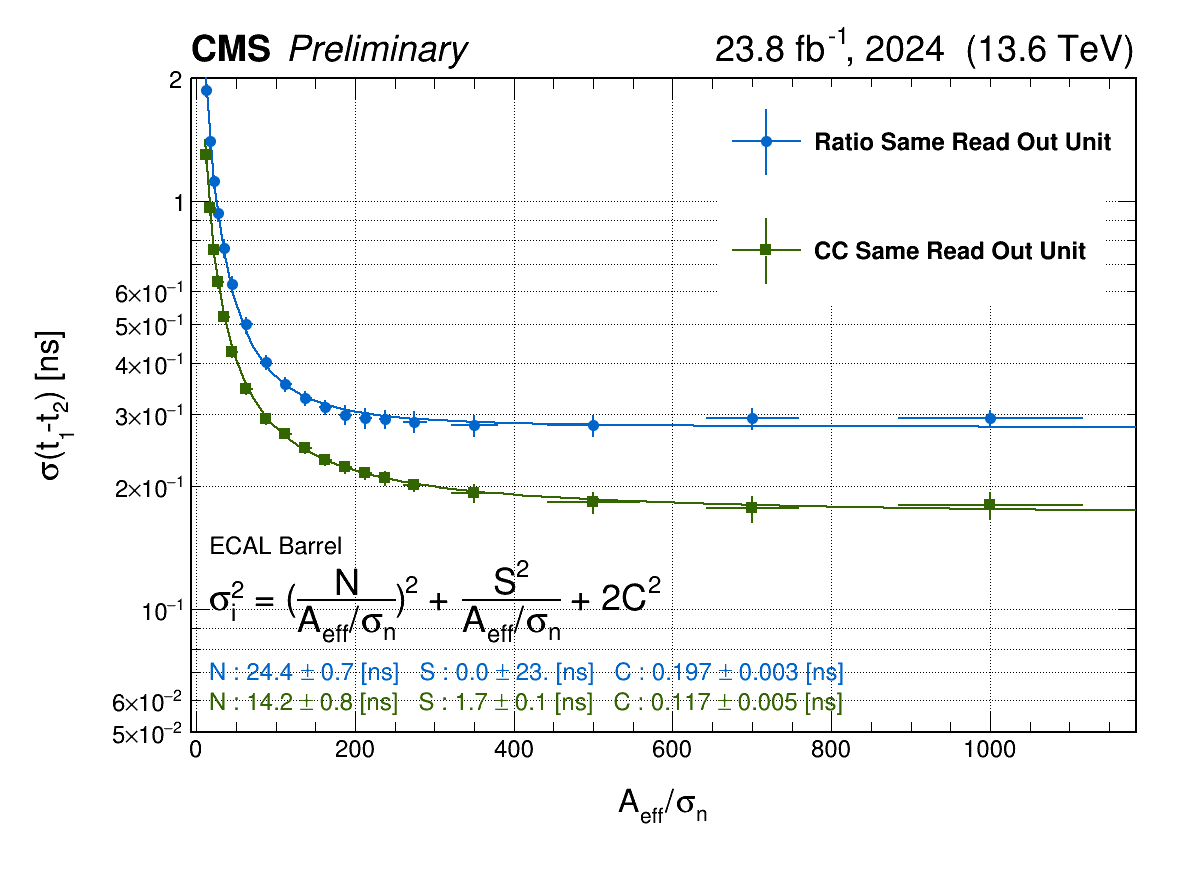
\includegraphics{fig/sec_results/tr_hl_r3_24f_v2_rtvcc_xgs_07082025170637.png}}
\caption{Comparison of same readout unit (SRU) and $Z \rightarrow e^{+}e^{-}$ object-level (ZEE) timing resolutions for the ratio and CC algorithms in Run~III.
The results are obtained from two independent prompt reconstructions of the same dataset.
An improvement of approximately 80~ps in the SRU resolution is observed for the CC algorithm.}
\label{ccresr3}
\end{center}
\end{figure}

A particularly informative comparison is provided by data collected during the 2024F data-taking period.
In this era, two independent prompt reconstructions of the same dataset were produced using official online CMS calibrations, differing only in the choice of the default ECAL timing reconstruction algorithm.
One reconstruction employed the ratio-based timing method, while the other used the CC algorithm as the default time reconstruction.
This configuration enables a direct comparison of the two timing algorithms under identical detector conditions, calibration strategies, and pileup environments, without relying on external or offline reprocessing.

The timing resolutions obtained in the 2024F data-taking period are shown in Fig.~\ref{ccresr2024F}.
A clear improvement is observed when the CC algorithm is used as the default ECAL timing reconstruction in prompt reconstruction.
Relative to the ratio-based method, the CC algorithm achieves a significantly improved same readout unit (SRU) resolution, together with a corresponding improvement in the $Z \rightarrow e^{+}e^{-}$ object-level (ZEE) timing resolution.
These results demonstrate that the performance gains observed in earlier two-tier studies persist when the CC algorithm is deployed as the default timing reconstruction within the full CMS prompt reconstruction chain using official online calibrations.
In the 2024F era, the CC reconstruction improves the SRU resolution by approximately XX~ps and the ZEE resolution by approximately YY~ps relative to the ratio-based reconstruction.

% added plots
\begin{figure}[h!tbp]
\begin{center}
\resizebox{0.7\textwidth}{!}{\includegraphics{fig/sec_results/tr_rtvcc_2024F_prompt_placeholder.png} }
\caption{Comparison of same readout unit (SRU) and $Z \rightarrow e^{+}e^{-}$ object-level (ZEE) timing resolutions obtained during prompt reconstruction in the 2024F data-taking period.
Two independent prompt reconstructions of the same dataset are compared, one using the ratio-based timing algorithm and the other using the CC algorithm as the default ECAL time reconstruction, both with official online CMS calibrations.
The CC algorithm exhibits improved SRU and ZEE timing resolutions relative to the ratio-based reconstruction.}
\label{ccresr2024F}
\end{center}
\end{figure}

Figure~\ref{ccresr4} shows the timing performance of the CC algorithm during the 2025 Run~III data-taking period, in which the CC reconstruction was used exclusively as the default ECAL timing algorithm for prompt reconstruction, together with its corresponding online calibration.
In this configuration, the CC algorithm achieves an SRU resolution of approximately 135~ps and a ZEE resolution of approximately 180~ps in prompt reconstruction.
Comparing the ZEE resolution achieved with the CC algorithm to the SRU resolution obtained with the ratio algorithm in Run~III demonstrates that the CC reconstruction substantially mitigates the impact of OOT-PU on analysis-relevant timing performance.
These improvements directly enhance the sensitivity of analyses relying on ECAL timing, particularly in high-pileup environments.

\begin{figure}[h!tbp]
\begin{center}
\resizebox{0.7\textwidth}{!}{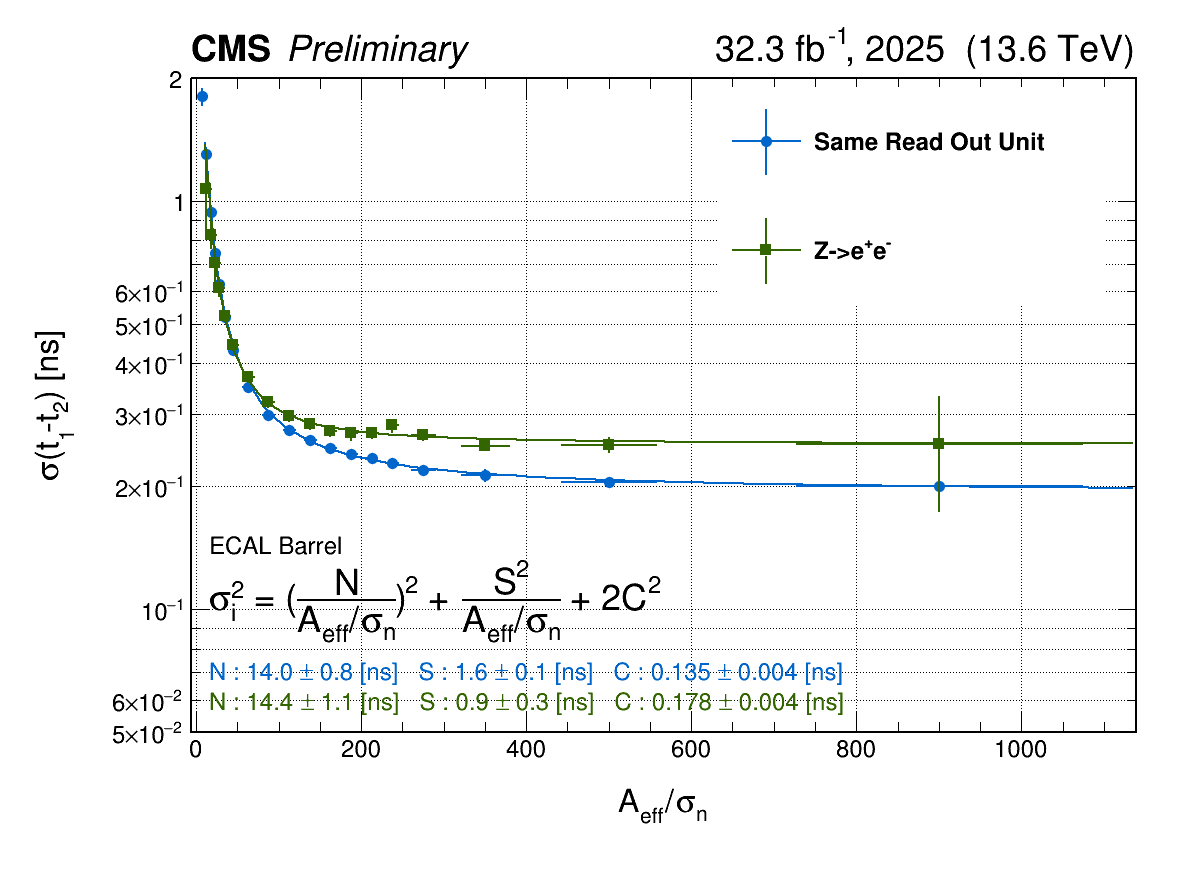
\includegraphics{fig/sec_results/tr_hl_r3_25c2_08082025165318.png}}
\caption{Same readout unit (SRU) and $Z \rightarrow e^{+}e^{-}$ object-level (ZEE) timing resolutions obtained with the CC algorithm during prompt reconstruction in Run~III (2025).
The CC algorithm, together with a dedicated online calibration, achieves an SRU resolution of approximately 135~ps and a ZEE resolution of approximately 180~ps.}
\label{ccresr4}
\end{center}
\end{figure}
%redone
\FloatBarrier

\section{Summary \label{sec:conclusion}}
In the High-Luminosity LHC (HL-LHC) era, the instantaneous luminosity is expected to increase by approximately a factor of five relative to current LHC operating conditions.
While these conditions will enable the accumulation of datasets more than an order of magnitude larger than those collected in all preceding LHC runs, they will also substantially increase the number of pileup interactions per event.
To mitigate the resulting degradation of event reconstruction performance, both the CMS and ATLAS experiments are incorporating precision timing measurements into their detectors through a combination of new sub-detectors and upgrades to existing systems, including the electromagnetic calorimeter (ECAL).
These developments enable four-dimensional (4D) event reconstruction techniques that provide powerful tools for pileup suppression and enhanced sensitivity to a wide range of physics signatures, including those involving long-lived particles.

The CMS ECAL, through the fast scintillation response of PbWO$_4$ crystals, the characteristics of the front-end electronics, and the readout sampling rate, is capable of achieving excellent intrinsic timing resolution.
However, ECAL timing reconstruction is sensitive to contributions from pileup interactions, particularly out-of-time pileup (OOT-PU), which becomes a dominant limitation as luminosity increases.
As part of the ECAL performance program, a target timing resolution of approximately 30~ps has been established for HL-LHC operation.
In preparation for these conditions, methods to mitigate the impact of OOT-PU on ECAL timing reconstruction have been studied.

In this work, a cross-correlation (CC) timing reconstruction algorithm is presented.
The CC algorithm exploits the out-of-time pulse amplitudes determined by the pileup-aware multi-fit energy reconstruction together with the known characteristic pulse shape of scintillation signals.
By reconstructing the nominal in-time pulse contribution and determining the pulse time via a cross-correlation with the pulse template, the CC algorithm significantly mitigates the effects of OOT-PU and improves the ECAL timing resolution.

Studies of the mean rechit time as a function of bunch-crossing position demonstrate that the CC algorithm substantially reduces both the dependence of the reconstructed time on bunch-crossing position and the energy dependence of the timing measurement.
In direct comparisons using Run~II data, the CC algorithm improves the same readout unit (SRU) timing resolution by approximately 30~ps and the $Z \rightarrow e^{+}e^{-}$ object-level (ZEE) timing resolution by approximately 35~ps relative to the default ratio-based reconstruction.

In Run~III, the CC algorithm was fully integrated into the CMS software framework and a dedicated online timing calibration was deployed.
A dedicated prompt reconstruction using the CC algorithm as the default ECAL timing method demonstrates an improvement of approximately 80~ps in the SRU resolution relative to the ratio-based reconstruction.
During early Run~III data-taking in 2025, the CC algorithm achieved an SRU resolution of approximately 135~ps and a ZEE resolution of approximately 180~ps in prompt reconstruction.
Based on this demonstrated performance, the CC timing reconstruction was adopted as the default ECAL timing algorithm for CMS data taking in 2025.

With continued operation in Run~III, comparable or improved timing performance is expected.
The CC reconstruction provides a robust and scalable framework for ECAL timing in high-pileup environments and establishes a solid foundation for future precision timing applications in the HL-LHC era.

\FloatBarrier

\pagebreak
\FloatBarrier
\medskip
\printbibliography[heading=bibnumbered,title={References}] 
%Prints the entire bibliography with the titel "Whole bibliography"

\end{document}

